% Options for packages loaded elsewhere
\PassOptionsToPackage{unicode}{hyperref}
\PassOptionsToPackage{hyphens}{url}
\PassOptionsToPackage{dvipsnames,svgnames,x11names}{xcolor}
\documentclass[
  british,
  10pt,
  a4paper,
]{article}
\usepackage{xcolor}
\usepackage[margin=20mm]{geometry}
\usepackage{amsmath,amssymb}
\setcounter{secnumdepth}{5}
\usepackage{iftex}
\ifPDFTeX
  \usepackage[T1]{fontenc}
  \usepackage[utf8]{inputenc}
  \usepackage{textcomp} % provide euro and other symbols
\else % if luatex or xetex
  \usepackage{unicode-math} % this also loads fontspec
  \defaultfontfeatures{Scale=MatchLowercase}
  \defaultfontfeatures[\rmfamily]{Ligatures=TeX,Scale=1}
\fi
\usepackage{lmodern}
\ifPDFTeX\else
  % xetex/luatex font selection
\fi
% Use upquote if available, for straight quotes in verbatim environments
\IfFileExists{upquote.sty}{\usepackage{upquote}}{}
\IfFileExists{microtype.sty}{% use microtype if available
  \usepackage[]{microtype}
  \UseMicrotypeSet[protrusion]{basicmath} % disable protrusion for tt fonts
}{}
\makeatletter
\@ifundefined{KOMAClassName}{% if non-KOMA class
  \IfFileExists{parskip.sty}{%
    \usepackage{parskip}
  }{% else
    \setlength{\parindent}{0pt}
    \setlength{\parskip}{6pt plus 2pt minus 1pt}}
}{% if KOMA class
  \KOMAoptions{parskip=half}}
\makeatother
\usepackage{listings}
\newcommand{\passthrough}[1]{#1}
\lstset{defaultdialect=[5.3]Lua}
\lstset{defaultdialect=[x86masm]Assembler}
\usepackage{longtable,booktabs,array}
\usepackage{calc} % for calculating minipage widths
% Correct order of tables after \paragraph or \subparagraph
\usepackage{etoolbox}
\makeatletter
\patchcmd\longtable{\par}{\if@noskipsec\mbox{}\fi\par}{}{}
\makeatother
% Allow footnotes in longtable head/foot
\IfFileExists{footnotehyper.sty}{\usepackage{footnotehyper}}{\usepackage{footnote}}
\makesavenoteenv{longtable}
\usepackage{graphicx}
\makeatletter
\newsavebox\pandoc@box
\newcommand*\pandocbounded[1]{% scales image to fit in text height/width
  \sbox\pandoc@box{#1}%
  \Gscale@div\@tempa{\textheight}{\dimexpr\ht\pandoc@box+\dp\pandoc@box\relax}%
  \Gscale@div\@tempb{\linewidth}{\wd\pandoc@box}%
  \ifdim\@tempb\p@<\@tempa\p@\let\@tempa\@tempb\fi% select the smaller of both
  \ifdim\@tempa\p@<\p@\scalebox{\@tempa}{\usebox\pandoc@box}%
  \else\usebox{\pandoc@box}%
  \fi%
}
% Set default figure placement to htbp
\def\fps@figure{htbp}
\makeatother
\ifLuaTeX
\usepackage[bidi=basic,shorthands=off,]{babel}
\else
\usepackage[bidi=default,shorthands=off,]{babel}
\fi
\ifLuaTeX
  \usepackage{selnolig} % disable illegal ligatures
\fi
\setlength{\emergencystretch}{3em} % prevent overfull lines
\providecommand{\tightlist}{%
  \setlength{\itemsep}{0pt}\setlength{\parskip}{0pt}}
% Shared print styling; prose and results live in the Markdown source.
\usepackage{amsmath}
\usepackage{microtype}
\usepackage{float}
\usepackage{needspace}
\usepackage{fancyhdr}
\usepackage{etoolbox}
\usepackage{caption}
\definecolor{labblue}{HTML}{0072B2}
\definecolor{laborange}{HTML}{D55E00}
\definecolor{codebg}{HTML}{F4F6F8}
\AtBeginDocument{\hypersetup{linkcolor=labblue,urlcolor=labblue,citecolor=labblue,pageanchor=false}}
\lstset{
  basicstyle=\fontsize{9}{10.5}\selectfont\ttfamily,
  keywordstyle=\color{labblue}\bfseries,
  commentstyle=\color{black!55},
  stringstyle=\color{laborange},
  backgroundcolor=\color{codebg},
  frame=single,rulecolor=\color{black!12},
  breaklines=true,breakatwhitespace=false,
  columns=fullflexible,keepspaces=true,
  showstringspaces=false,tabsize=4,
  xleftmargin=5pt,xrightmargin=5pt,
  aboveskip=10pt,belowskip=10pt
}
\captionsetup{font=small,labelfont=bf}
\floatplacement{figure}{htbp}
\renewcommand{\topfraction}{0.9}
\renewcommand{\bottomfraction}{0.8}
\renewcommand{\textfraction}{0.1}
\renewcommand{\floatpagefraction}{0.75}
\pagestyle{fancy}
\fancyhf{}
\fancyhead[L]{\small\textcolor{labblue}{LABFIT / PRACTICAL TUTORIAL}}
\fancyhead[R]{\small Synthetic laboratory data}
\fancyfoot[C]{\small\thepage}
\setlength{\headheight}{15pt}
\setlength{\emergencystretch}{3em}
\setlength{\parskip}{4pt}
\raggedbottom
\let\labtoc\tableofcontents
\renewcommand{\tableofcontents}{\begingroup\small\labtoc\endgroup}
\makeatletter
\renewcommand{\maketitle}{
  \begin{titlepage}
  \thispagestyle{empty}
  \vspace*{8mm}
  {\Large\bfseries\color{labblue} LABFIT\par}
  \vspace{5mm}
  {\large A practical laboratory tutorial\par}
  \vspace{10mm}
  {\fontsize{28}{32}\selectfont\bfseries\raggedright\hyphenpenalty=10000\@title\par}
  \vspace{8mm}
  {\Large Fitting, uncertainty and diagnostics\par}
  \vspace{10mm}
  \begin{center}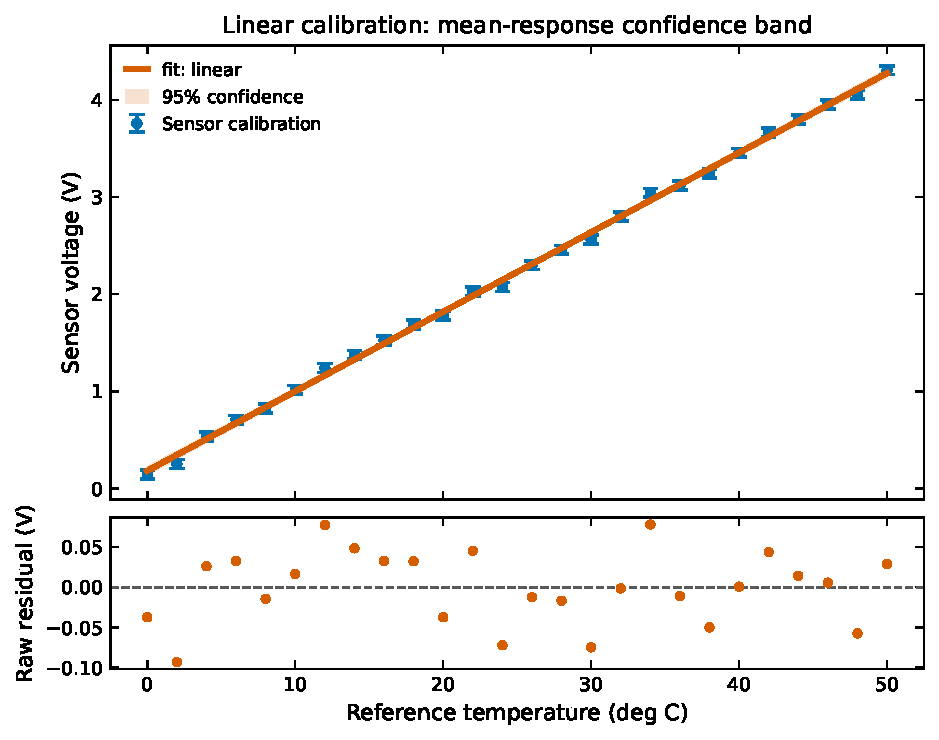
\includegraphics[width=0.95\textwidth,height=80mm,keepaspectratio]{figures/01_calibration.pdf}\end{center}
  \vfill
  {\large Six experiments. One reproducible workflow.\par}
  \vspace{4mm}
  {\normalsize For undergraduate scientists with basic Python knowledge.\par}
  {\normalsize All measurements are synthetic and supplied with the tutorial.\par}
  \vspace{8mm}
  {\small LabFit 0.2.0 \hfill October 2026\par}
  \end{titlepage}
\hypersetup{pageanchor=true}
}
\makeatother
\usepackage{bookmark}
\IfFileExists{xurl.sty}{\usepackage{xurl}}{} % add URL line breaks if available
\urlstyle{same}
\hypersetup{
  pdftitle={From First Fit to Advanced Laboratory Analysis},
  pdfauthor={LabFit practical tutorial},
  pdflang={en-GB},
  colorlinks=true,
  linkcolor={Maroon},
  filecolor={Maroon},
  citecolor={Blue},
  urlcolor={Blue},
  pdfcreator={LaTeX via pandoc}}

\title{From First Fit to Advanced Laboratory Analysis}
\author{LabFit practical tutorial}
\date{October 2026}

\begin{document}
\maketitle

{
\hypersetup{linkcolor=}
\setcounter{tocdepth}{2}
\tableofcontents
}
\clearpage

\section{Getting started}\label{getting-started}

\Needspace{8\baselineskip}

\subsection{What you will learn}\label{what-you-will-learn}

A useful laboratory fit connects a physical question to a mathematical
model, measured observations, and an honest account of uncertainty.
Drawing a smooth curve is one part of that process. Deciding whether the
model explains the observations, and whether the reported parameter
errors are credible, takes more care.

This tutorial introduces that workflow using \textbf{LabFit}, a Python
library built on NumPy, SciPy and Matplotlib. You will analyse six
synthetic experiments, moving from a straight-line calibration to
overlapping peaks and correlated measurement errors. Every example
includes an executable script, the observations, figures, fitted results
and an interpretation.

The intended reader knows basic Python variables, functions and arrays,
and has met measurement uncertainty in a laboratory course. You do not
need prior experience with nonlinear optimisation. The mathematics is
introduced alongside the code that uses it.

\begin{longtable}[]{@{}
  >{\raggedright\arraybackslash}p{(\linewidth - 4\tabcolsep) * \real{0.3333}}
  >{\raggedright\arraybackslash}p{(\linewidth - 4\tabcolsep) * \real{0.3333}}
  >{\raggedright\arraybackslash}p{(\linewidth - 4\tabcolsep) * \real{0.3333}}@{}}
\toprule\noalign{}
\begin{minipage}[b]{\linewidth}\raggedright
Stage
\end{minipage} & \begin{minipage}[b]{\linewidth}\raggedright
Experiment
\end{minipage} & \begin{minipage}[b]{\linewidth}\raggedright
New capability
\end{minipage} \\
\midrule\noalign{}
\endhead
\bottomrule\noalign{}
\endlastfoot
Simple & Sensor calibration & CSV loading, linear fitting, prediction \\
Simple & Signal decay & Nonlinear fitting, derived half-life \\
Intermediate & Single spectral peak & Background terms, bounds,
covariance propagation \\
Intermediate & Repeated oscillations & Independent fits to multiple
series \\
Complex & Overlapping spectral peaks & Custom model, multiple starts,
correlations \\
Complex & Thermal response & Generalized least squares, whitened
residuals \\
\end{longtable}

Read the examples in sequence on a first pass. Later, use the individual
scripts as starting points for your own analysis. These experiments are
illustrative; \textbf{no real instrument or material was measured}. The
generating truth is available for validation, but the analysis scripts
do not read it to choose fitted values.

\Needspace{8\baselineskip}

\subsection{Install the current
checkout}\label{install-the-current-checkout}

The tutorial follows the interfaces in this repository. LabFit requires
Python 3.10 or later. Install this checkout into an isolated environment
so that the examples and the library version agree.

\par\noindent\begin{minipage}{\linewidth}

\begin{lstlisting}[language=sh]
git clone https://github.com/matthewjdoyle/labfit.git
cd labfit
python -m venv .venv
\end{lstlisting}

\end{minipage}\par

Activate the environment using the command for your platform:

\par\noindent\begin{minipage}{\linewidth}

\begin{lstlisting}[language=sh]
# Windows PowerShell
.venv\Scripts\Activate.ps1

# macOS or Linux
source .venv/bin/activate
\end{lstlisting}

\end{minipage}\par

Then install and run the demonstrations:

\par\noindent\begin{minipage}{\linewidth}

\begin{lstlisting}[language=sh]
python -m pip install -e .
python examples/tutorial/run_examples.py
\end{lstlisting}

\end{minipage}\par

The run creates or refreshes the figures and
\passthrough{\lstinline!results.json!}. It uses a non-interactive
Matplotlib backend, so you do not need to close plot windows. A warning
about the Gaussian model in Example 3 is expected: that example
deliberately fits an incomplete model to reveal its limitations.

The supplied document was built using \textbf{labfit 0.2.0, numpy 2.2.6,
scipy 1.15.2, matplotlib 3.10.1}. Small differences in the final digits
can occur with other supported numerical-library versions. Interpret
uncertainties and physical scales rather than demanding identical
floating-point results across every platform.

\Needspace{8\baselineskip}

\subsection{Orient yourself in the tutorial
package}\label{orient-yourself-in-the-tutorial-package}

Keep the files in \passthrough{\lstinline!examples/tutorial/!} together.
The directory contains:

\begin{longtable}[]{@{}
  >{\raggedright\arraybackslash}p{(\linewidth - 2\tabcolsep) * \real{0.5000}}
  >{\raggedright\arraybackslash}p{(\linewidth - 2\tabcolsep) * \real{0.5000}}@{}}
\toprule\noalign{}
\begin{minipage}[b]{\linewidth}\raggedright
Item
\end{minipage} & \begin{minipage}[b]{\linewidth}\raggedright
Purpose
\end{minipage} \\
\midrule\noalign{}
\endhead
\bottomrule\noalign{}
\endlastfoot
\passthrough{\lstinline!data/*.csv!} & Observations, with explicit
measurement errors \\
\passthrough{\lstinline!data/manifest.json!} & Seeds, units, equations,
noise assumptions and generating truth \\
\passthrough{\lstinline!example\_01\_*.py!} through
\passthrough{\lstinline!example\_06\_*.py!} & Complete executable
analyses \\
\passthrough{\lstinline!common.py!} & Figure-saving and reporting
helpers \\
\passthrough{\lstinline!figures/!} & PNG images for reading and vector
PDF images for printing \\
\passthrough{\lstinline!results.json!} & Full computed results,
including fitted covariance \\
\passthrough{\lstinline!tutorial.md!},
\passthrough{\lstinline!tutorial.tex!},
\passthrough{\lstinline!tutorial.pdf!} & The three presentation
formats \\
\end{longtable}

The code excerpts below are drawn directly from the executable scripts.
They show the analysis within each script's
\passthrough{\lstinline!run!} function. The complete files contain the
imports, reporting and plotting helpers needed to execute them.

For an interactive session, start with these common imports and paths:

\par\noindent\begin{minipage}{\linewidth}

\begin{lstlisting}[language=Python]
from pathlib import Path
import numpy as np
from labfit import fit, fit_multi, plot_fit, plot_multi_fit
from labfit.io import load_csv
from labfit.utils import propagate_errors

data = Path("examples/tutorial/data")  # from the repository root
\end{lstlisting}

\end{minipage}\par

Use \passthrough{\lstinline!plot.save("my\_fit.png")!} to save a LabFit
plot. The tutorial's \passthrough{\lstinline!save\_figure!} helper saves
both PNG and PDF and closes the figure; the helper is a convenience for
this package, rather than part of LabFit.

\Needspace{8\baselineskip}

\subsection{Start with the
observations}\label{start-with-the-observations}

The basic CSV layout is deliberately simple:

\par\noindent\begin{minipage}{\linewidth}

\begin{lstlisting}
x,y,sigma
0.0,0.19,0.045
2.0,0.35,0.045
\end{lstlisting}

\end{minipage}\par

These two rows illustrate the format; the actual measured values appear
in the worked examples. Here \passthrough{\lstinline!sigma!} means the
standard deviation of measurement noise in \textbf{y}, in the same units
as y. It is not a variance, percentage, or confidence-interval width.
The standard CSV reader recognises this column.

\par\noindent\begin{minipage}{\linewidth}

\begin{lstlisting}[language=Python]
series = load_csv(data / "calibration.csv")
print(series.x.shape, series.y.shape)
print(series.sigma)
\end{lstlisting}

\end{minipage}\par

LabFit can also fit arrays directly, accept a CSV path, or use a
\passthrough{\lstinline!DataSeries!} object that carries data, a label
and an uncertainty specification. Loading first is useful when you want
to inspect observations before committing to a model.

All x values in these experiments are treated as exact. If your
reference temperatures, wavelengths or times have appreciable
uncertainty, that assumption needs examination. The examples do not
demonstrate errors-in-variables fitting.

\clearpage

\section{The fitting workflow}\label{the-fitting-workflow}

\Needspace{8\baselineskip}

\subsection{State a model and a noise
assumption}\label{state-a-model-and-a-noise-assumption}

Write a model \(M(x;\boldsymbol{\theta})\) that represents the expected
response. The vector \(\boldsymbol{\theta}\) contains the parameters to
estimate. A linear calibration, for example, has slope and intercept.

The observed response differs from the model by a residual:

\begin{equation}r_i = y_i - M(x_i;\hat{\boldsymbol{\theta}}).\end{equation}

The hat denotes fitted parameters. This definition matches
\passthrough{\lstinline!result.residuals!}: observations minus fitted
predictions.

For independent Gaussian measurement errors with known standard
deviations \(s_i\), weighted least squares minimises

\begin{equation}\chi^2(\boldsymbol{\theta})
= \sum_{i=1}^{N}\left[\frac{y_i-M(x_i;\boldsymbol{\theta})}{s_i}\right]^2.\end{equation}

The \textbf{standardized residual} \(z_i=r_i/s_i\) is dimensionless. A
raw residual of 0.1 V might be small for one instrument and enormous for
another; standardized residuals let you judge it against its stated
error. LabFit's default residual panel displays \textbf{raw residuals},
so this tutorial labels those panels with units.

The supplied data use known Gaussian noise scales. We therefore
consistently pass \passthrough{\lstinline!absolute\_sigma=True!}. That
choice affects the reported parameter covariance; it does not change the
optimum for a fixed model and error specification.

\Needspace{8\baselineskip}

\subsection{Read the result before trusting the
curve}\label{read-the-result-before-trusting-the-curve}

\par\noindent\begin{minipage}{\linewidth}

\begin{lstlisting}[language=Python]
result = fit(series, model="linear", absolute_sigma=True)
print(result)
print(result.params)
print(result.uncertainties)

if not result.success:
    raise RuntimeError(result.message)
if not result.identifiable:
    raise RuntimeError("The observations do not distinguish every parameter.")
\end{lstlisting}

\end{minipage}\par

\passthrough{\lstinline!success!} reports whether the optimiser
converged. \passthrough{\lstinline!identifiable!} reports a local
Jacobian diagnostic: whether changes in the parameters produce
sufficiently distinct changes in the predicted observations. A model can
converge even when several parameters can trade off without changing its
predictions.

For \(N\) observations and \(k\) free parameters, the degrees of freedom
are

\begin{equation}\nu=N-k,\qquad \chi^2_\nu=\frac{\chi^2}{\nu}.\end{equation}

Under an appropriate model and calibrated independent Gaussian errors,
reduced chi-square is expected to fluctuate around one. A rough
fluctuation scale is \(\sqrt{2/\nu}\) for the linear Gaussian setting.
Thus 1.1 may be unremarkable for a small experiment and more noteworthy
for thousands of observations.

A large value can indicate omitted structure, underestimated errors or
outliers. A small value can indicate overestimated errors, unusual
sampling fluctuations or an overly flexible model. The statistic alone
cannot identify the cause. Inspect the residuals and revisit how the
measurements were made.

The chi-square p-value is the upper-tail probability of obtaining a
chi-square at least this large under the assumed model and error
specification. It is \textbf{not the probability that the model is
true}. Nonlinear fits use a local approximation, and fitted bounds or
model-selection steps can complicate the interpretation further.

\Needspace{8\baselineskip}

\subsection{Parameter errors and two different
covariances}\label{parameter-errors-and-two-different-covariances}

LabFit stores fitted parameter covariance in
\passthrough{\lstinline!result.covariance!}, with its rows and columns
ordered by \passthrough{\lstinline!result.param\_names!}. Standard
errors are the square roots of the diagonal entries. These are local
estimates around the optimum; strong nonlinearity, active bounds or
inadequate data can make a symmetric error summary misleading.

Use different symbols for two different objects:

\begin{longtable}[]{@{}
  >{\raggedright\arraybackslash}p{(\linewidth - 4\tabcolsep) * \real{0.3333}}
  >{\raggedright\arraybackslash}p{(\linewidth - 4\tabcolsep) * \real{0.3333}}
  >{\raggedright\arraybackslash}p{(\linewidth - 4\tabcolsep) * \real{0.3333}}@{}}
\toprule\noalign{}
\begin{minipage}[b]{\linewidth}\raggedright
Symbol
\end{minipage} & \begin{minipage}[b]{\linewidth}\raggedright
Meaning
\end{minipage} & \begin{minipage}[b]{\linewidth}\raggedright
Dimensions
\end{minipage} \\
\midrule\noalign{}
\endhead
\bottomrule\noalign{}
\endlastfoot
\(C_y\) & Covariance between measurement errors & \(N\times N\) \\
\(C_\theta\) & Covariance between fitted parameter estimates &
\(k\times k\) \\
\end{longtable}

The thermal experiment supplies \(C_y\) through
\passthrough{\lstinline!sigma\_cov!}. The fitting result provides
\(C_\theta\). You cannot substitute one for the other.

For a weighted residual Jacobian \(J\), a locally full-rank model has
approximately

\begin{equation}C_\theta^{\mathrm{absolute}}=(J^T J)^{-1},\qquad
C_\theta^{\mathrm{relative}}=C_\theta^{\mathrm{absolute}}\,\chi^2_\nu.\end{equation}

The default \passthrough{\lstinline!absolute\_sigma=False!} uses the
supplied errors as relative weights and estimates a common scale from
residual scatter. Use that policy when only the relative weighting is
justified. In these synthetic experiments, the supplied sigmas are
calibrated absolute uncertainties, so rescaling them from residuals
would discard known information.

\Needspace{8\baselineskip}

\subsection{Missing uncertainties and unweighted
analysis}\label{missing-uncertainties-and-unweighted-analysis}

If a CSV omits error columns, LabFit can infer heuristic uncertainties
and emits a warning of type
\passthrough{\lstinline!UncertaintyInferenceWarning!}. The formula and
provenance are stored on the loaded series. A heuristic is an
exploratory assumption; it does not turn missing measurement knowledge
into a calibrated error model.

For an explicitly unweighted analysis:

\par\noindent\begin{minipage}{\linewidth}

\begin{lstlisting}[language=Python]
unweighted = load_csv(data / "calibration.csv", error_mode="unweighted")
relative_result = fit(unweighted, model="linear")
print(relative_result.residual_variance)
\end{lstlisting}

\end{minipage}\par

This example intentionally ignores the supplied error column to
illustrate the interface. An unweighted result does not have meaningful
weighted chi-square or chi-square p-value; these fields are NaN. Use
\passthrough{\lstinline!residual\_variance!}, the raw residual sum of
squares divided by positive degrees of freedom, to describe scatter in
squared y units.

Supply exactly one fitting error specification:
\passthrough{\lstinline!sigma!}, inverse-variance
\passthrough{\lstinline!weights!}, an asymmetric pair, or
\passthrough{\lstinline!sigma\_cov!}. These demonstrations use symmetric
errors and covariance. For asymmetric inputs, LabFit retains both sides
for plotting and fits using an effective root-mean-square sigma; this is
an approximation rather than a full asymmetric likelihood.

\clearpage

\section{Simple example 1: linear sensor
calibration}\label{simple-example-1-linear-sensor-calibration}

\Needspace{8\baselineskip}

\subsection{Question and model}\label{question-and-model}

A temperature sensor returns a voltage. We compare it with a reference
temperature over a controlled range and ask: \textbf{what voltage
response should we expect at a given temperature, and how uncertain is
that mean response?}

The model is

\begin{equation}V(T)=mT+b.\end{equation}

\begin{longtable}[]{@{}llll@{}}
\toprule\noalign{}
Parameter & LabFit name & Meaning & Unit \\
\midrule\noalign{}
\endhead
\bottomrule\noalign{}
\endlastfoot
\(m\) & \passthrough{\lstinline!slope!} & Sensitivity & V/degree C \\
\(b\) & \passthrough{\lstinline!intercept!} & Voltage at 0 degree C &
V \\
\end{longtable}

The synthetic experiment contains 26 evenly spaced temperatures from 0
to 50 degrees C. The generator uses \(m=0.082\) V/degree C and
\(b=0.18\) V, then adds independent Gaussian voltage noise with standard
deviation 0.045 V. The seed is 101. The reference temperatures are
treated as exact.

The first observations in \href{data/calibration.csv}{the calibration
CSV} are:

\begin{longtable}[]{@{}lll@{}}
\toprule\noalign{}
x & y & sigma \\
\midrule\noalign{}
\endhead
\bottomrule\noalign{}
\endlastfoot
0 & 0.144443 & 0.045 \\
2 & 0.252442 & 0.045 \\
4 & 0.535149 & 0.045 \\
6 & 0.705493 & 0.045 \\
8 & 0.822064 & 0.045 \\
\end{longtable}

\Needspace{8\baselineskip}

\subsection{Load, fit and predict}\label{load-fit-and-predict}

Run the complete example:

\par\noindent\begin{minipage}{\linewidth}

\begin{lstlisting}[language=sh]
python examples/tutorial/example_01_calibration.py
\end{lstlisting}

\end{minipage}\par

The script's analysis is:

\par\noindent\begin{minipage}{\linewidth}

\begin{lstlisting}[language=Python]
series = load_csv(data / "calibration.csv", label="Sensor calibration")
result = fit(series, model="linear", absolute_sigma=True)
temperature = 25.0
prediction = float(result.predict([temperature])[0])
gradient = np.array([temperature, 1.0])  # slope, intercept
prediction_error = float(np.sqrt(gradient @ result.covariance @ gradient))

confidence = plot_fit(
    result,
    show_ci=True,
    ci_level=0.95,
    xlabel="Reference temperature (deg C)",
    ylabel="Sensor voltage (V)",
    title="Linear calibration: mean-response confidence band",
)
raw_labels(confidence, "V")
save_figure(confidence, "01_calibration", figures)
future = plot_fit(
    result,
    show_ci=True,
    prediction=True,
    ci_level=0.95,
    prediction_sigma=0.045,
    xlabel="Reference temperature (deg C)",
    ylabel="Sensor voltage (V)",
    title="Linear calibration: future-observation prediction band",
)
raw_labels(future, "V")
save_figure(future, "01_prediction", figures)
\end{lstlisting}

\end{minipage}\par

The call to \passthrough{\lstinline!fit!} returns the slope and
intercept. \passthrough{\lstinline!predict!} evaluates the attached
model using the fitted parameters. It can take an array of temperatures,
so the same method supports a single prediction or a dense plotting
grid.

For a prediction at \(T_*\), the gradient with respect to \((m,b)\) is
\(\boldsymbol{g}=(T_*,1)^T\). Its mean-response uncertainty is

\begin{equation}s_{\mathrm{mean}}(T_*) =
\sqrt{\boldsymbol{g}^T C_\theta \boldsymbol{g}}.\end{equation}

The off-diagonal covariance between slope and intercept is part of this
calculation. Simply adding the separate parameter-error contributions in
quadrature can give a different answer.

\Needspace{8\baselineskip}

\subsection{Results and residuals}\label{results-and-residuals}

\begin{longtable}[]{@{}llll@{}}
\toprule\noalign{}
Parameter & Estimate & Standard error & Unit \\
\midrule\noalign{}
\endhead
\bottomrule\noalign{}
\endlastfoot
\passthrough{\lstinline!slope!} & 0.0818358 & 0.000588 & V/degree C \\
\passthrough{\lstinline!intercept!} & 0.18191 & 0.0172 & V \\
\end{longtable}

Degrees of freedom: \textbf{24}; reduced chi-square: \textbf{1.074};
chi-square p-value: \textbf{0.3645}. Converged: \textbf{True};
identifiable: \textbf{True}.

\begin{longtable}[]{@{}llll@{}}
\toprule\noalign{}
Derived quantity & Estimate & Standard error & Unit \\
\midrule\noalign{}
\endhead
\bottomrule\noalign{}
\endlastfoot
Mean voltage at 25 deg C & 2.2278 & 0.00883 & V \\
\end{longtable}

\begin{figure}
\centering
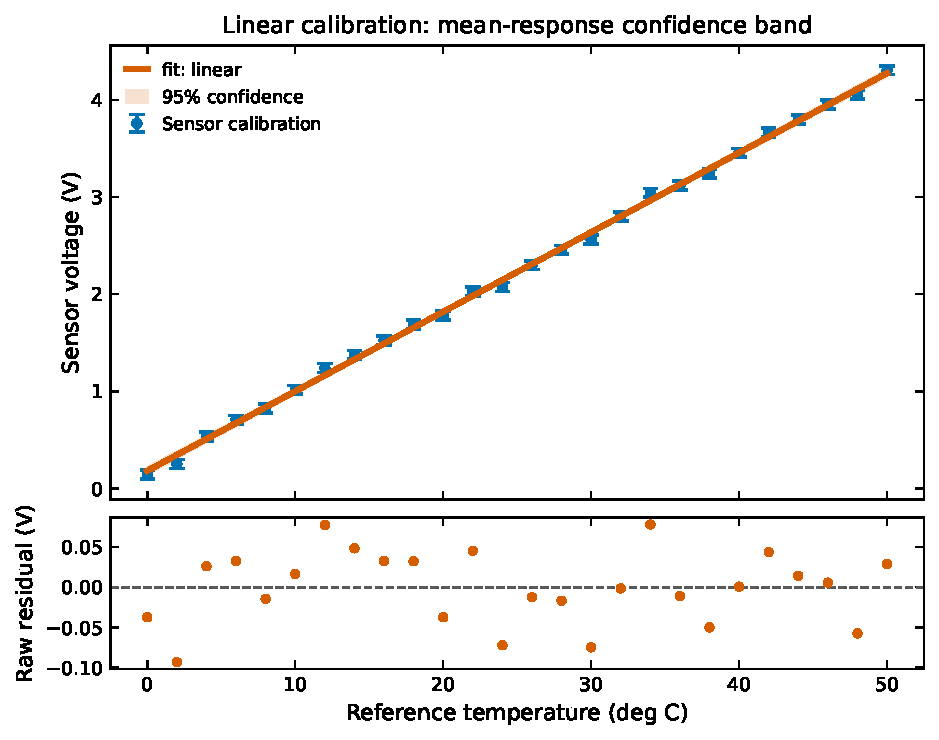
\includegraphics[width=0.9\linewidth,height=\textheight,keepaspectratio]{figures/01_calibration.pdf}
\caption{Linear sensor calibration. Error bars show
one-standard-deviation measurement errors. The shaded region is a
pointwise 95 percent confidence band for the mean voltage; the lower
panel shows raw residuals in volts.}
\end{figure}

The estimated sensitivity is close to the generating value. The
residuals fluctuate around zero without a strong systematic trend, and
their scale is consistent with the supplied errors. Reduced chi-square
and its p-value support that reading of the plot; neither replaces
inspection of the data.

The prediction at 25 degrees C is interpolation within the experiment.
It is usually safer than extrapolating beyond the measured range, where
unmodelled curvature or sensor saturation may become relevant.

\Needspace{8\baselineskip}

\subsection{Mean response versus a future
reading}\label{mean-response-versus-a-future-reading}

There are two distinct questions: how uncertain is the estimated mean
voltage, and how variable will a single new measurement be? A new
independent reading contains both mean-response uncertainty and
measurement noise.

\begin{equation}s_{\mathrm{future}}^2(T_*) =
s_{\mathrm{mean}}^2(T_*) + s_{\mathrm{new}}^2.\end{equation}

The second plot passes the new reading's noise explicitly with
\passthrough{\lstinline!prediction\_sigma=0.045!}. That number is an
absolute standard deviation in volts. It is never rescaled by reduced
chi-square when passed explicitly.

\begin{figure}
\centering
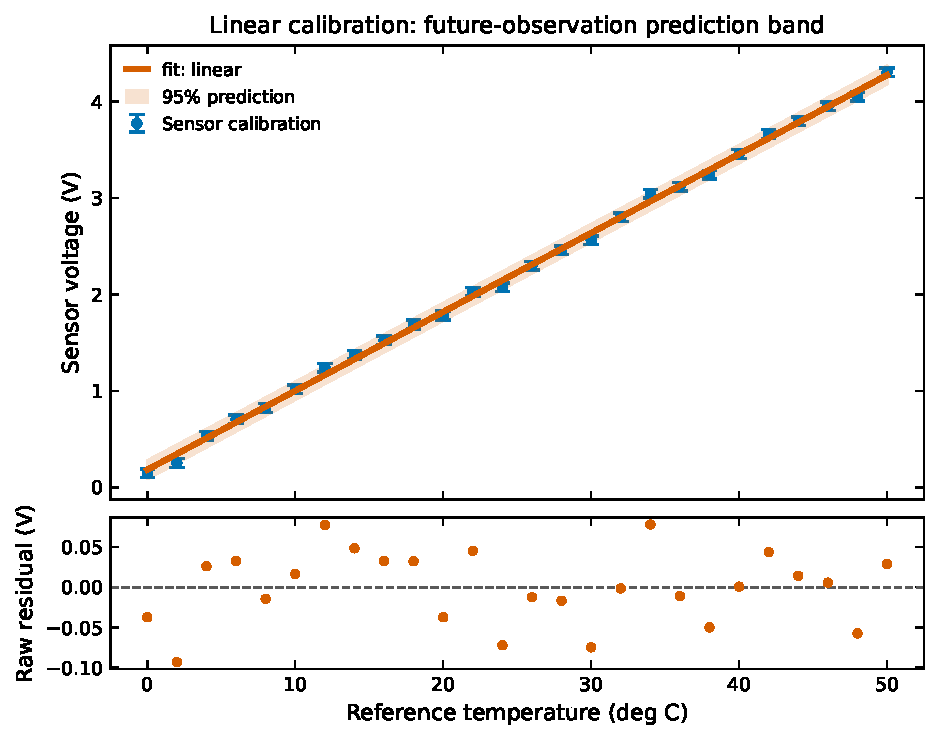
\includegraphics[width=0.9\linewidth,height=\textheight,keepaspectratio]{figures/01_prediction.pdf}
\caption{Prediction band for a future independent calibration reading.
It is wider than the mean-response confidence band because it includes
new measurement noise.}
\end{figure}

Both bands use \textbf{pointwise normal approximations}. A 95 percent
pointwise band does not promise that an entire future curve will stay
inside it with 95 percent probability. The prediction calculation also
assumes that the new error is independent of the measurements used to
estimate the parameters.

\textbf{Laboratory lesson:} report whether a band describes a fitted
mean or a future observation. A precise mean estimate does not eliminate
instrument noise in the next reading.

\clearpage

\section{Simple example 2: exponential signal
decay}\label{simple-example-2-exponential-signal-decay}

\Needspace{8\baselineskip}

\subsection{Question and model}\label{question-and-model-1}

After a source is switched off, a signal decreases with time. We ask:
\textbf{what decay rate describes the signal, and what is the
corresponding half-life?}

LabFit's \passthrough{\lstinline!exponential!} model uses a decay rate,
rather than a time constant:

\begin{equation}S(t)=A\exp(-\lambda t).\end{equation}

\begin{longtable}[]{@{}llll@{}}
\toprule\noalign{}
Parameter & LabFit name & Meaning & Unit \\
\midrule\noalign{}
\endhead
\bottomrule\noalign{}
\endlastfoot
\(A\) & \passthrough{\lstinline!amplitude!} & Signal at zero time & V \\
\(\lambda\) & \passthrough{\lstinline!decay!} & Decay rate & 1/s \\
\end{longtable}

The 49 synthetic observations span 0 to 12 seconds. The generating
values are \(A=4.8\) V and \(\lambda=0.24\) per second. Independent
Gaussian noise has standard deviation 0.075 V, and the seed is 202.
There is no additive background in this experiment; this assumption is
part of the model.

The first rows of \href{data/decay.csv}{the decay CSV} are:

\begin{longtable}[]{@{}lll@{}}
\toprule\noalign{}
x & y & sigma \\
\midrule\noalign{}
\endhead
\bottomrule\noalign{}
\endlastfoot
0 & 4.93588 & 0.075 \\
0.25 & 4.46579 & 0.075 \\
0.5 & 4.1758 & 0.075 \\
0.75 & 3.97915 & 0.075 \\
1 & 3.68937 & 0.075 \\
\end{longtable}

\Needspace{8\baselineskip}

\subsection{Choose an initial
estimate}\label{choose-an-initial-estimate}

A nonlinear model benefits from a physically plausible initial estimate.
Here the first reading estimates the amplitude. Two well-separated
readings that remain positive give an approximate rate:

\begin{equation}\lambda_0 \approx
\frac{\log[S(0)/S(t_1)]}{t_1}.\end{equation}

This estimate only starts the optimiser. The final fit minimises the
residuals in the original voltage units, using all observations and
their sigmas.

Taking logarithms of the entire noisy dataset and fitting a straight
line would change the error model. Constant voltage noise becomes
nonconstant, asymmetric noise after the logarithm, and negative readings
cannot be logged. The initial estimate does not make that transformation
the fitting objective.

\Needspace{8\baselineskip}

\subsection{Execute the analysis}\label{execute-the-analysis}

\par\noindent\begin{minipage}{\linewidth}

\begin{lstlisting}[language=sh]
python examples/tutorial/example_02_decay.py
\end{lstlisting}

\end{minipage}\par

\par\noindent\begin{minipage}{\linewidth}

\begin{lstlisting}[language=Python]
series = load_csv(data / "decay.csv", label="Decaying signal")
# Estimate a rate from two well-separated, still-positive readings.
midpoint = len(series.y) // 2
rate_guess = np.log(series.y[0] / series.y[midpoint]) / series.x[midpoint]
result = fit(
    series,
    model="exponential",
    absolute_sigma=True,
    p0={"amplitude": float(series.y[0]), "decay": float(rate_guess)},
    bounds={"amplitude": (0, None), "decay": (0.001, 2)},
)
half_life, half_life_error = propagate_errors(
    lambda decay: np.log(2.0) / decay,
    jacobian=lambda decay: -np.log(2.0) / decay**2,
    decay=result.params["decay"],
    decay_error=result.uncertainties["decay"],
)
plot = plot_fit(
    result,
    show_ci=True,
    ci_level=0.95,
    xlabel="Time (s)",
    ylabel="Signal voltage (V)",
    title="Exponential signal decay",
)
raw_labels(plot, "V")
save_figure(plot, "02_decay", figures)
\end{lstlisting}

\end{minipage}\par

Bounds enforce positive amplitude and rate. The supplied starting values
lie inside the bounds. On a different dataset, verify positive starting
estimates and appropriate physical ranges before using this recipe.

\Needspace{8\baselineskip}

\subsection{Derive the half-life}\label{derive-the-half-life}

The half-life \(t_{1/2}\) is the time needed to halve the noiseless
signal:

\begin{equation}t_{1/2}=\frac{\log 2}{\lambda},\qquad
s_{t_{1/2}} =
\left|\frac{-\log 2}{\lambda^2}\right|s_\lambda.\end{equation}

\passthrough{\lstinline!propagate\_errors!} evaluates the derived
function and uses its gradient to propagate uncertainty. This particular
quantity depends only on the rate, so one parameter's standard error is
sufficient. A quantity depending on both amplitude and rate should
retain their covariance.

\begin{longtable}[]{@{}llll@{}}
\toprule\noalign{}
Parameter & Estimate & Standard error & Unit \\
\midrule\noalign{}
\endhead
\bottomrule\noalign{}
\endlastfoot
\passthrough{\lstinline!amplitude!} & 4.81192 & 0.0352 & V \\
\passthrough{\lstinline!decay!} & 0.239178 & 0.00264 & 1/s \\
\end{longtable}

Degrees of freedom: \textbf{47}; reduced chi-square: \textbf{1.083};
chi-square p-value: \textbf{0.3225}. Converged: \textbf{True};
identifiable: \textbf{True}.

\begin{longtable}[]{@{}llll@{}}
\toprule\noalign{}
Derived quantity & Estimate & Standard error & Unit \\
\midrule\noalign{}
\endhead
\bottomrule\noalign{}
\endlastfoot
Half-life & 2.89804 & 0.032 & s \\
\end{longtable}

\begin{figure}
\centering
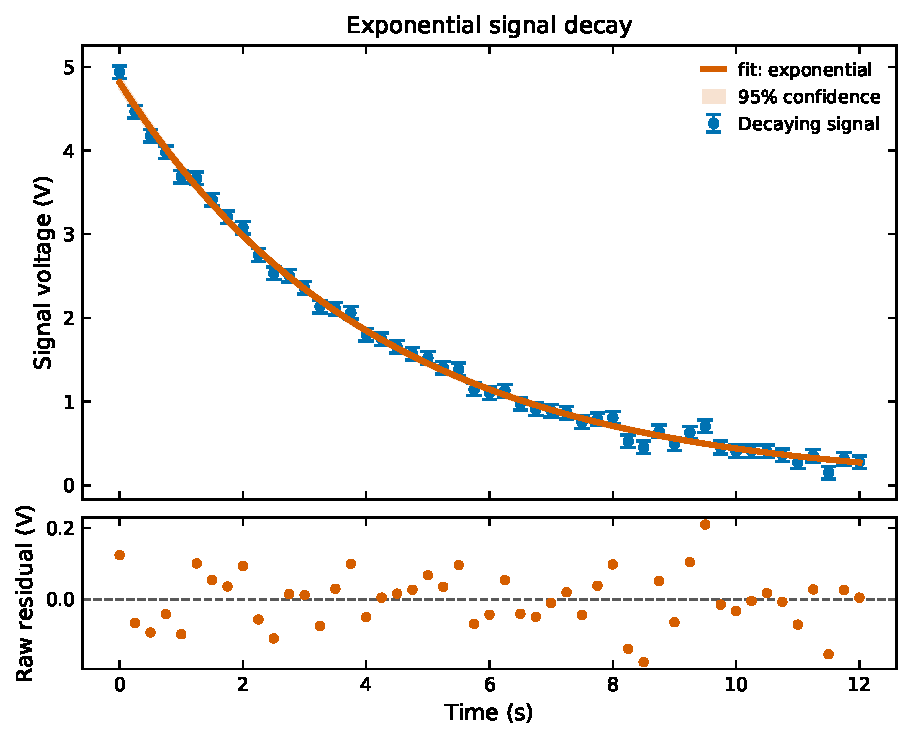
\includegraphics[width=0.9\linewidth,height=\textheight,keepaspectratio]{figures/02_decay.pdf}
\caption{Exponential voltage decay with a pointwise 95 percent
confidence band. Raw residuals remain on the voltage scale; the fitted
half-life is derived from the decay rate.}
\end{figure}

The half-life is close to the generating value \(\log 2/0.24\), about
2.89 seconds. The confidence band describes the fitted mean decay,
rather than the likely spread of a new voltage reading.

\Needspace{8\baselineskip}

\subsection{Assess the physical
assumptions}\label{assess-the-physical-assumptions}

A systematic tail in the residuals could indicate an unmodelled
background, multiple decay components, or a time-dependent noise scale.
A small standard error on \(\lambda\) would not repair those
shortcomings.

The first-order error formula is appropriate when the local parameter
uncertainty is small enough for linearisation. If the rate is close to
zero, or a bound is active, half-life uncertainty can become strongly
asymmetric. Then a symmetric value-plus-error summary needs additional
analysis.

\textbf{Laboratory lesson:} make the parameterisation explicit. A decay
rate has units of inverse time; a time constant and half-life have units
of time. Confusing them can produce a plausible-looking but physically
wrong report.

\clearpage

\section{Intermediate example 3: a peak on a sloping
background}\label{intermediate-example-3-a-peak-on-a-sloping-background}

\Needspace{8\baselineskip}

\subsection{Question and model}\label{question-and-model-2}

A spectral peak sits above a slowly changing baseline. We ask:
\textbf{what are its centre, width and integrated signal once the
background is accounted for?}

Work in a wavelength offset \(u=\lambda_{\mathrm{wavelength}}-550\) nm:

\begin{equation}I(u)=A\exp\left[-\frac{1}{2}
\left(\frac{u-\mu}{w}\right)^2\right]+mu+b.\end{equation}

The slope symbol \(m\) is unrelated to the calibration experiment's
slope. LabFit calls the Gaussian width parameter
\passthrough{\lstinline!sigma!}; the symbol \(w\) here keeps it distinct
from measurement sigmas \(s_i\).

\begin{longtable}[]{@{}lll@{}}
\toprule\noalign{}
LabFit name & Meaning & Unit \\
\midrule\noalign{}
\endhead
\bottomrule\noalign{}
\endlastfoot
\passthrough{\lstinline!amplitude!} & Peak height above baseline & mV \\
\passthrough{\lstinline!mean!} & Peak centre relative to 550 nm & nm \\
\passthrough{\lstinline!sigma!} & Gaussian width & nm \\
\passthrough{\lstinline!m!} & Background slope & mV/nm \\
\passthrough{\lstinline!b!} & Background at zero offset & mV \\
\end{longtable}

There are 141 observations over offsets from -3.5 to 3.5 nm. The
generator uses amplitude 2.8 mV, centre 0.35 nm, width 0.62 nm, slope
0.12 mV/nm and baseline 0.7 mV. Noise is independent Gaussian with
known, varying standard deviation

\begin{equation}s_i = 0.045 + 0.018\sqrt{I_{\mathrm{true}}(u_i)}\end{equation}

when numerical signal values are expressed in mV. The coefficients
define a synthetic noise prescription, rather than a detector law. Seed
303 fixes the random draws. Each supplied sigma is a calibrated noise
scale, not an estimate made from its individual noisy observation.

The first rows of \href{data/single_peak.csv}{the single-peak CSV} are:

\begin{longtable}[]{@{}lll@{}}
\toprule\noalign{}
x & y & sigma \\
\midrule\noalign{}
\endhead
\bottomrule\noalign{}
\endlastfoot
-3.5 & 0.23812 & 0.0545247 \\
-3.45 & 0.261617 & 0.0546262 \\
-3.4 & 0.244144 & 0.0547267 \\
-3.35 & 0.310927 & 0.0548261 \\
-3.3 & 0.266807 & 0.0549245 \\
\end{longtable}

\Needspace{8\baselineskip}

\subsection{Estimate a background before
fitting}\label{estimate-a-background-before-fitting}

The far wings contain little peak signal. A straight-line estimate using
these points gives a useful background start. Subtracting that
provisional background makes it easier to estimate the peak height and
centre.

This subtraction is used to obtain initial values. The final fit jointly
estimates all five parameters using the original observations. Treating
a noisy background estimate as exact and fitting only a subtracted peak
would lose uncertainty information.

\par\noindent\begin{minipage}{\linewidth}

\begin{lstlisting}[language=sh]
python examples/tutorial/example_03_single_peak.py
\end{lstlisting}

\end{minipage}\par

\par\noindent\begin{minipage}{\linewidth}

\begin{lstlisting}[language=Python]
series = load_csv(data / "single_peak.csv", label="Peak plus background")
edge = np.abs(series.x) > 2.5
slope, intercept = np.polyfit(series.x[edge], series.y[edge], 1)
corrected = series.y - slope * series.x - intercept
centre = float(series.x[np.argmax(corrected)])
result = fit(
    series,
    model="gaussian_baseline",
    absolute_sigma=True,
    p0={
        "amplitude": float(corrected.max()),
        "mean": centre,
        "sigma": 0.7,
        "m": float(slope),
        "b": float(intercept),
    },
    bounds={"amplitude": (0, None), "mean": (-1.5, 1.5), "sigma": (0.1, 2)},
)
wrong = fit(
    series,
    model="gaussian",
    absolute_sigma=True,
    p0={"amplitude": float(series.y.max()), "mean": centre, "sigma": 0.7},
    bounds={"amplitude": (0, None), "mean": (-1.5, 1.5), "sigma": (0.1, 4)},
)
\end{lstlisting}

\end{minipage}\par

A positive width bound prevents a zero-width singularity. The centre
bounds identify the region of interest. Bounds encode assumptions and
should be justifiable from the experiment; they are not a substitute for
informative data.

\Needspace{8\baselineskip}

\subsection{Inspect the complete and incomplete
models}\label{inspect-the-complete-and-incomplete-models}

\begin{longtable}[]{@{}llll@{}}
\toprule\noalign{}
Parameter & Estimate & Standard error & Unit \\
\midrule\noalign{}
\endhead
\bottomrule\noalign{}
\endlastfoot
\passthrough{\lstinline!amplitude!} & 2.77298 & 0.0204 & mV \\
\passthrough{\lstinline!mean!} & 0.353109 & 0.00497 & nm \\
\passthrough{\lstinline!sigma!} & 0.625423 & 0.00529 & nm \\
\passthrough{\lstinline!m!} & 0.123636 & 0.00262 & mV/nm \\
\passthrough{\lstinline!b!} & 0.698024 & 0.00707 & mV \\
\end{longtable}

Degrees of freedom: \textbf{136}; reduced chi-square: \textbf{1.044};
chi-square p-value: \textbf{0.3448}. Converged: \textbf{True};
identifiable: \textbf{True}.

\begin{figure}
\centering
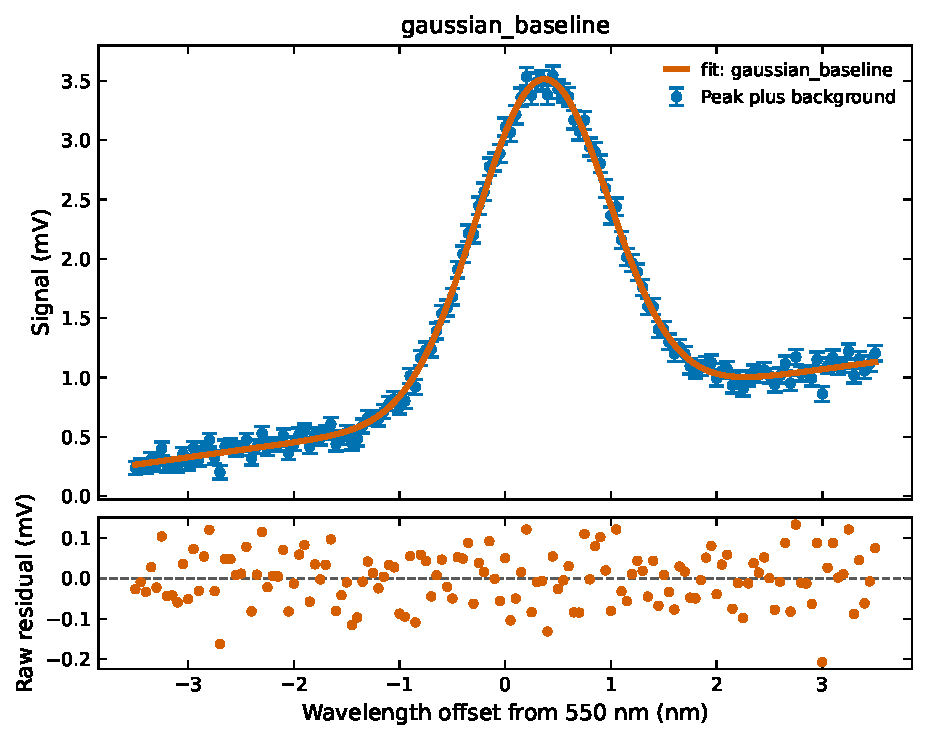
\includegraphics[width=0.9\linewidth,height=\textheight,keepaspectratio]{figures/03_single_peak.pdf}
\caption{Gaussian peak with a fitted sloping baseline. The residual
panel is on the raw signal scale and shows no strong remaining
background structure.}
\end{figure}

For comparison, the script fits \passthrough{\lstinline!gaussian!}
without any background parameters. That optimiser can converge, but it
must absorb the baseline into its peak.

\begin{longtable}[]{@{}llll@{}}
\toprule\noalign{}
Parameter & Estimate & Standard error & Unit \\
\midrule\noalign{}
\endhead
\bottomrule\noalign{}
\endlastfoot
\passthrough{\lstinline!amplitude!} & 2.75936 & 0.0137 & mV \\
\passthrough{\lstinline!mean!} & 0.533883 & 0.00619 & nm \\
\passthrough{\lstinline!sigma!} & 1.2252 & 0.00618 & nm \\
\end{longtable}

Degrees of freedom: \textbf{138}; reduced chi-square: \textbf{47.77};
chi-square p-value: \textbf{0}. Converged: \textbf{True}; identifiable:
\textbf{True}.

The reported p-value of zero reflects floating-point underflow;
interpret it as extremely small.

\begin{figure}
\centering
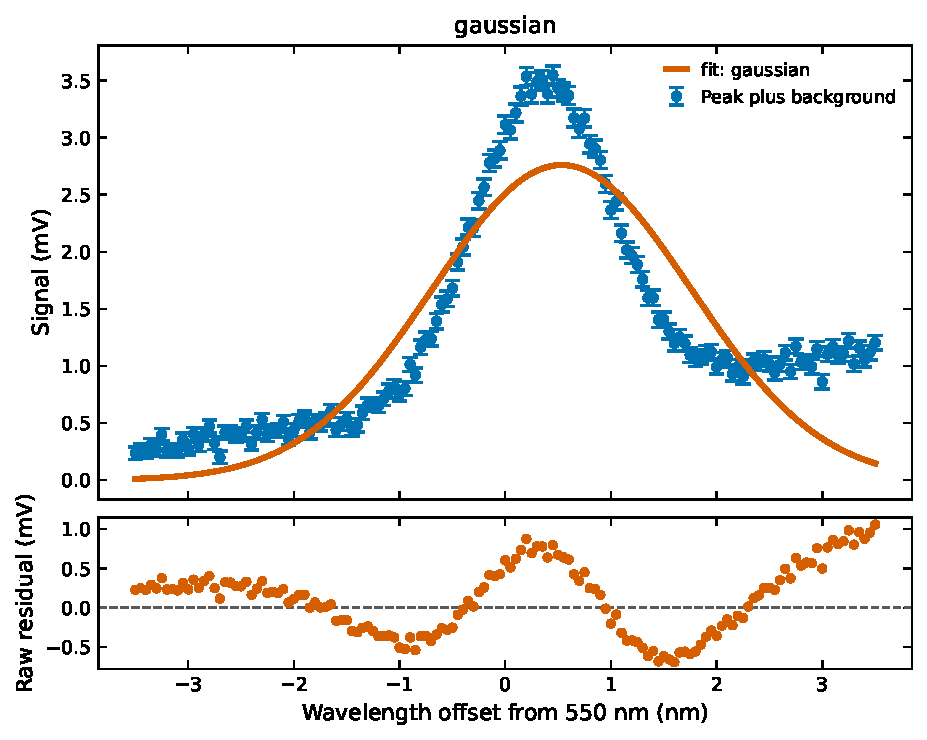
\includegraphics[width=0.9\linewidth,height=\textheight,keepaspectratio]{figures/03_missing_background.pdf}
\caption{Background-free Gaussian fitted to observations that contain a
sloping baseline. The residual trend reveals systematic model
inadequacy, despite optimiser convergence.}
\end{figure}

Reduced chi-square changes from \textbf{47.7745} for the background-free
model to \textbf{1.04417} for the complete model. The visual evidence
also matters: the incomplete model leaves a coherent residual pattern
across wavelength.

Adding parameters generally improves a least-squares objective. That
fact alone does not establish that the larger model is physically
correct. Here the background is motivated by the experiment, residual
structure disappears, and the calibrated-error diagnostic becomes
plausible.

Because errors vary between observations, standardized residuals are
more informative about the noise assumption:

\par\noindent\begin{minipage}{\linewidth}

\begin{lstlisting}[language=Python]
standardized = result.residuals / result.sigma
\end{lstlisting}

\end{minipage}\par

\begin{figure}
\centering
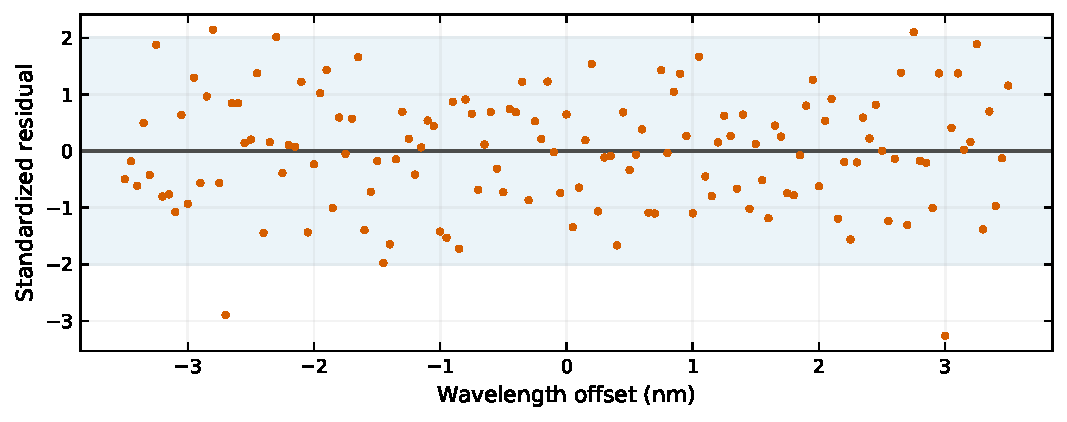
\includegraphics[width=0.9\linewidth,height=\textheight,keepaspectratio]{figures/03_standardized.pdf}
\caption{Standardized residuals for the peak-plus-background model. The
shaded region marks plus or minus two measurement standard deviations as
a visual guide; it is not a simultaneous acceptance region.}
\end{figure}

Do not expect every standardized residual to lie within two. Fitted
residuals also have leverage effects and are not exactly independent
standard normal draws, even when the underlying measurement errors are
independent.

\Needspace{8\baselineskip}

\subsection{Width and integrated peak
area}\label{width-and-integrated-peak-area}

Two quantities are useful for a spectral report. The full width at half
maximum and the baseline-subtracted area of an ideal Gaussian are

\begin{equation}\mathrm{FWHM}=2\sqrt{2\log 2}\,w,\qquad
Q=\sqrt{2\pi}\,Aw.\end{equation}

\(Q\) integrates the fitted Gaussian over the entire real line. It
excludes the baseline, and it is not the area of the full signal within
the measured window. Its units are mV nm.

Amplitude and width can trade off, so their covariance contributes to
the area uncertainty:

\begin{equation}s_Q^2 =
2\pi\left[w^2s_A^2+A^2s_w^2+2Aw\,\mathrm{Cov}(A,w)\right].\end{equation}

Extract the relevant parameter covariance in the same order as the
arguments to the derived function:

\par\noindent\begin{minipage}{\linewidth}

\begin{lstlisting}[language=Python]
indices = [result.param_names.index(name) for name in ("amplitude", "sigma")]
area_covariance = result.covariance[np.ix_(indices, indices)]
area, area_error = propagate_errors(
    lambda amplitude, sigma: np.sqrt(2 * np.pi) * amplitude * sigma,
    jacobian=lambda amplitude, sigma: np.sqrt(2 * np.pi) * np.array([sigma, amplitude]),
    covariance=area_covariance,
    amplitude=result.params["amplitude"],
    sigma=result.params["sigma"],
)
factor = 2 * np.sqrt(2 * np.log(2))
fwhm = factor * result.params["sigma"]
fwhm_error = factor * result.uncertainties["sigma"]
\end{lstlisting}

\end{minipage}\par

\begin{longtable}[]{@{}llll@{}}
\toprule\noalign{}
Derived quantity & Estimate & Standard error & Unit \\
\midrule\noalign{}
\endhead
\bottomrule\noalign{}
\endlastfoot
FWHM & 1.47276 & 0.0125 & nm \\
Integrated peak area & 4.34722 & 0.0381 & mV nm \\
\end{longtable}

\passthrough{\lstinline!np.ix\_!} selects both the relevant rows and
columns. Selecting parameters in one order and passing values or a
gradient in another would propagate the wrong uncertainty without
necessarily producing an obvious exception.

\textbf{Laboratory lesson:} the background is part of the uncertainty
problem. Joint fitting and covariance propagation preserve the
relationships between background, height and width.

\clearpage

\section{Intermediate example 4: repeated damped
oscillations}\label{intermediate-example-4-repeated-damped-oscillations}

\Needspace{8\baselineskip}

\subsection{Question and model}\label{question-and-model-3}

Three runs record a damped oscillation. We ask: \textbf{how do the
estimated frequency and damping compare across runs?}

Use the built-in sine-form model with an offset:

\begin{equation}d(t)=d_0+A\exp(-\gamma t)\sin(2\pi f t+\phi).\end{equation}

\begin{longtable}[]{@{}lll@{}}
\toprule\noalign{}
LabFit name & Meaning & Unit \\
\midrule\noalign{}
\endhead
\bottomrule\noalign{}
\endlastfoot
\passthrough{\lstinline!amplitude!} & Initial envelope amplitude & mm \\
\passthrough{\lstinline!damping!} & Envelope decay rate & 1/s \\
\passthrough{\lstinline!frequency!} & Cycles per second & Hz \\
\passthrough{\lstinline!phase!} & Initial phase & rad \\
\passthrough{\lstinline!offset!} & Equilibrium displacement & mm \\
\end{longtable}

Frequency is in cycles per second because the model supplies \(2\pi\).
Using an angular frequency in this parameter would introduce a
factor-of-\(2\pi\) error.

Each run has 161 samples over 0 to 8 seconds, with independent Gaussian
noise of standard deviation 0.10 mm. The seeds are 401, 402 and 403. The
generator uses slightly different parameters in each run:

\begin{longtable}[]{@{}
  >{\raggedright\arraybackslash}p{(\linewidth - 10\tabcolsep) * \real{0.1667}}
  >{\raggedright\arraybackslash}p{(\linewidth - 10\tabcolsep) * \real{0.1667}}
  >{\raggedright\arraybackslash}p{(\linewidth - 10\tabcolsep) * \real{0.1667}}
  >{\raggedright\arraybackslash}p{(\linewidth - 10\tabcolsep) * \real{0.1667}}
  >{\raggedright\arraybackslash}p{(\linewidth - 10\tabcolsep) * \real{0.1667}}
  >{\raggedright\arraybackslash}p{(\linewidth - 10\tabcolsep) * \real{0.1667}}@{}}
\toprule\noalign{}
\begin{minipage}[b]{\linewidth}\raggedright
Run
\end{minipage} & \begin{minipage}[b]{\linewidth}\raggedright
Amplitude (mm)
\end{minipage} & \begin{minipage}[b]{\linewidth}\raggedright
Damping (1/s)
\end{minipage} & \begin{minipage}[b]{\linewidth}\raggedright
Frequency (Hz)
\end{minipage} & \begin{minipage}[b]{\linewidth}\raggedright
Phase (rad)
\end{minipage} & \begin{minipage}[b]{\linewidth}\raggedright
Offset (mm)
\end{minipage} \\
\midrule\noalign{}
\endhead
\bottomrule\noalign{}
\endlastfoot
1 & 3.1 & 0.17 & 0.88 & 0.20 & 0.12 \\
2 & 2.8 & 0.19 & 0.90 & 0.35 & 0.08 \\
3 & 3.3 & 0.16 & 0.87 & 0.10 & 0.15 \\
\end{longtable}

These generating settings describe this synthetic exercise. The fitted
values below are estimated from the observations.

The first observations in \href{data/oscillator_1.csv}{run 1} are:

\begin{longtable}[]{@{}lll@{}}
\toprule\noalign{}
x & y & sigma \\
\midrule\noalign{}
\endhead
\bottomrule\noalign{}
\endlastfoot
0 & 0.651141 & 0.1 \\
0.05 & 1.53981 & 0.1 \\
0.1 & 2.29473 & 0.1 \\
0.15 & 2.61083 & 0.1 \\
0.2 & 2.96572 & 0.1 \\
\end{longtable}

The other files are \href{data/oscillator_2.csv}{run 2} and
\href{data/oscillator_3.csv}{run 3}.

\Needspace{8\baselineskip}

\subsection{Obtain a frequency
estimate}\label{obtain-a-frequency-estimate}

For uniformly spaced time points, an FFT provides a useful starting
frequency. Subtract a provisional mean to reduce the zero-frequency
component, then select the largest nonzero spectral peak. This estimate
has limited resolution and can be affected by damping, sampling and
leakage. It is only a starting point for the time-domain fit.

The amplitude estimate comes from the observed range. An initial damping
of 0.1 per second is a rough envelope scale: it allows appreciable decay
across an eight-second run. It is not copied from the generator.

\par\noindent\begin{minipage}{\linewidth}

\begin{lstlisting}[language=sh]
python examples/tutorial/example_04_oscillators.py
\end{lstlisting}

\end{minipage}\par

\par\noindent\begin{minipage}{\linewidth}

\begin{lstlisting}[language=Python]
series = [load_csv(data / f"oscillator_{i}.csv", label=f"Run {i}") for i in range(1, 4)]
first = series[0]
centred = first.y - np.mean(first.y)
spectrum = np.abs(np.fft.rfft(centred))
frequencies = np.fft.rfftfreq(len(first.x), d=float(first.x[1] - first.x[0]))
frequency_guess = float(frequencies[1:][np.argmax(spectrum[1:])])
results = fit_multi(
    series,
    model="damped_sine",
    absolute_sigma=True,
    p0={
        "amplitude": float(np.ptp(first.y) / 2),
        "damping": 0.1,
        "frequency": frequency_guess,
        "phase": 0.0,
        "offset": float(first.y.mean()),
    },
    bounds={
        "amplitude": (0, 10),
        "damping": (0.001, 1),
        "frequency": (0.5, 1.3),
        "phase": (-np.pi, np.pi),
        "offset": (-1, 1),
    },
)
plot = plot_multi_fit(results, series, figsize=(3.6, 3.7), xlabel="Time (s)", ylabel="Displacement (mm)")
raw_labels(plot, "mm")
save_figure(plot, "04_oscillators", figures)
\end{lstlisting}

\end{minipage}\par

\passthrough{\lstinline!load\_csv!} returns a
\passthrough{\lstinline!DataSeries!} for each run, carrying its label
and noise. \passthrough{\lstinline!fit\_multi!} uses the same model,
starting-value specification and bounds for every series.

It performs \textbf{three independent fits}. It does not estimate a
common frequency, share a damping parameter, or automatically pool the
experiments. A joint model with shared parameters is a different
analysis and is outside this example.

\Needspace{8\baselineskip}

\subsection{Compare the results}\label{compare-the-results}

\Needspace{6\baselineskip}

\subsubsection{Run 1}\label{run-1}

\begin{longtable}[]{@{}llll@{}}
\toprule\noalign{}
Parameter & Estimate & Standard error & Unit \\
\midrule\noalign{}
\endhead
\bottomrule\noalign{}
\endlastfoot
\passthrough{\lstinline!amplitude!} & 3.13589 & 0.03 & mm \\
\passthrough{\lstinline!damping!} & 0.170784 & 0.00314 & 1/s \\
\passthrough{\lstinline!frequency!} & 0.880153 & 0.00049 & Hz \\
\passthrough{\lstinline!phase!} & 0.198362 & 0.0095 & rad \\
\passthrough{\lstinline!offset!} & 0.110694 & 0.00793 & mm \\
\end{longtable}

Degrees of freedom: \textbf{156}; reduced chi-square: \textbf{0.9279};
chi-square p-value: \textbf{0.7305}. Converged: \textbf{True};
identifiable: \textbf{True}.

\Needspace{6\baselineskip}

\subsubsection{Run 2}\label{run-2}

\begin{longtable}[]{@{}llll@{}}
\toprule\noalign{}
Parameter & Estimate & Standard error & Unit \\
\midrule\noalign{}
\endhead
\bottomrule\noalign{}
\endlastfoot
\passthrough{\lstinline!amplitude!} & 2.75807 & 0.0301 & mm \\
\passthrough{\lstinline!damping!} & 0.185178 & 0.00371 & 1/s \\
\passthrough{\lstinline!frequency!} & 0.899372 & 0.000603 & Hz \\
\passthrough{\lstinline!phase!} & 0.364064 & 0.0112 & rad \\
\passthrough{\lstinline!offset!} & 0.0809072 & 0.00792 & mm \\
\end{longtable}

Degrees of freedom: \textbf{156}; reduced chi-square: \textbf{1.276};
chi-square p-value: \textbf{0.01127}. Converged: \textbf{True};
identifiable: \textbf{True}.

\Needspace{6\baselineskip}

\subsubsection{Run 3}\label{run-3}

\begin{longtable}[]{@{}llll@{}}
\toprule\noalign{}
Parameter & Estimate & Standard error & Unit \\
\midrule\noalign{}
\endhead
\bottomrule\noalign{}
\endlastfoot
\passthrough{\lstinline!amplitude!} & 3.31288 & 0.0297 & mm \\
\passthrough{\lstinline!damping!} & 0.160591 & 0.00284 & 1/s \\
\passthrough{\lstinline!frequency!} & 0.870806 & 0.000445 & Hz \\
\passthrough{\lstinline!phase!} & 0.0980559 & 0.00881 & rad \\
\passthrough{\lstinline!offset!} & 0.155297 & 0.00793 & mm \\
\end{longtable}

Degrees of freedom: \textbf{156}; reduced chi-square: \textbf{1.048};
chi-square p-value: \textbf{0.3242}. Converged: \textbf{True};
identifiable: \textbf{True}.

\begin{figure}
\centering
\pandocbounded{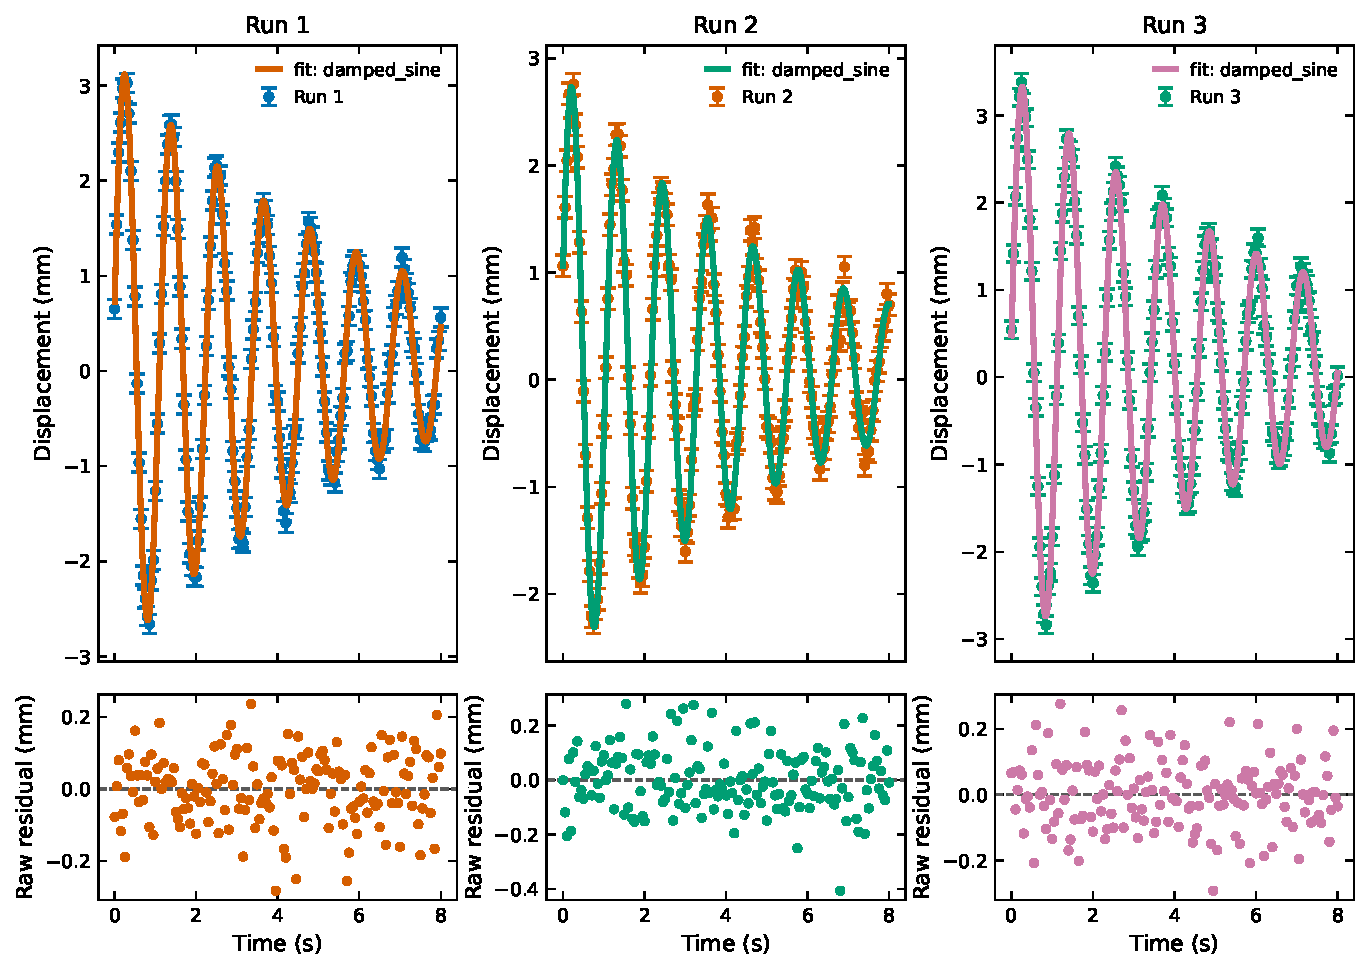
\includegraphics[keepaspectratio]{figures/04_oscillators.pdf}}
\caption{Independent damped-sine fits to three measurement runs. Each
column shows that run's observations, fitted curve and raw displacement
residuals.}
\end{figure}

Run 2 has an unusually large chi-square for its stated noise, even
though its observations were generated from the stated model. Such
fluctuations can occur. In a real experiment this would prompt careful
checks of the measurements and model, rather than automatic rejection or
error rescaling.

The fitted frequencies and damping rates differ across runs, as expected
from the generating settings. Parameter errors describe uncertainty
within each run's model; they do not automatically include variability
between experiments.

To assess a difference between independently estimated frequencies, a
first approximation is

\begin{equation}s_{f_1-f_2}=\sqrt{s_{f_1}^2+s_{f_2}^2}.\end{equation}

That expression assumes independence between the estimates. A common
clock calibration or shared systematic could invalidate it. Real repeats
may also contain experimental variation that is larger than the fitted
noise model.

\Needspace{8\baselineskip}

\subsection{Interpret residuals and
sampling}\label{interpret-residuals-and-sampling}

A repeated wave pattern in residuals can indicate the wrong frequency or
a missing mode. A slow drift can indicate a moving equilibrium. Large
early-time residuals may suggest the damping law is inadequate.

The evenly spaced time points make the FFT recipe convenient here. For
irregularly sampled data, do not pass an average time spacing into this
recipe and expect the same interpretation. Use a starting estimate
appropriate to the actual sampling or inspect the oscillations directly.

The model's fitted phase also depends on the time origin. Shifting time
zero changes phase, so phase comparisons require a consistent reference.

\textbf{Laboratory lesson:} distinguish the uncertainty of a fitted
parameter in one run from reproducibility across runs. Plotting several
experiments together helps reveal both, but it does not merge their
statistical models.

\clearpage

\section{Complex example 5: overlapping spectral
peaks}\label{complex-example-5-overlapping-spectral-peaks}

\Needspace{8\baselineskip}

\subsection{Question and custom model}\label{question-and-custom-model}

A spectrum contains two partly overlapping peaks and a background. We
ask: \textbf{can the data distinguish their centres, and how precisely
can we measure their separation?}

A single broad peak can resemble two narrow components. The difficulty
is therefore both numerical and statistical: a converged optimisation
may still leave strong parameter correlations.

The observations use absolute wavelengths from 548 to 553 nm. Define an
offset \(u=\lambda_{\mathrm{wavelength}}-550\) nm and model

\begin{equation}I(u)=
A_1\exp\left[-\frac{(u-c_1)^2}{2w_1^2}\right]
+A_2\exp\left[-\frac{(u-c_2)^2}{2w_2^2}\right]+mu+b.\end{equation}

\begin{longtable}[]{@{}lll@{}}
\toprule\noalign{}
Parameters & Meaning & Unit \\
\midrule\noalign{}
\endhead
\bottomrule\noalign{}
\endlastfoot
\passthrough{\lstinline!A1!}, \passthrough{\lstinline!A2!} & Peak
heights above baseline & mV \\
\passthrough{\lstinline!c1!}, \passthrough{\lstinline!c2!} & Centre
offsets from 550 nm & nm \\
\passthrough{\lstinline!w1!}, \passthrough{\lstinline!w2!} & Gaussian
widths & nm \\
\passthrough{\lstinline!m!} & Background slope & mV/nm \\
\passthrough{\lstinline!b!} & Background at 550 nm & mV \\
\end{longtable}

The 201 synthetic observations use peaks
\((A_1,c_1,w_1)=(2.5,-0.1,0.43)\) and \((A_2,c_2,w_2)=(1.8,0.8,0.52)\),
with background slope 0.06 mV/nm and intercept 0.35 mV. Noise is
independent Gaussian with standard deviation 0.055 mV; the seed is 505.

The first rows of \href{data/double_peak.csv}{the overlapping-peak CSV}
are:

\begin{longtable}[]{@{}lll@{}}
\toprule\noalign{}
x & y & sigma \\
\midrule\noalign{}
\endhead
\bottomrule\noalign{}
\endlastfoot
548 & 0.300096 & 0.055 \\
548.025 & 0.162814 & 0.055 \\
548.05 & 0.256456 & 0.055 \\
548.075 & 0.145247 & 0.055 \\
548.1 & 0.223257 & 0.055 \\
\end{longtable}

\Needspace{8\baselineskip}

\subsection{Define the function}\label{define-the-function}

LabFit accepts a custom callable. The first argument supplies x;
subsequent named arguments are fitted parameters. Return an array with
the same shape as the input.

\par\noindent\begin{minipage}{\linewidth}

\begin{lstlisting}[language=Python]
def double_peak(
    u: np.ndarray, A1: float, c1: float, w1: float, A2: float, c2: float, w2: float, m: float, b: float
) -> np.ndarray:
    first = A1 * np.exp(-0.5 * ((u - c1) / w1) ** 2)
    second = A2 * np.exp(-0.5 * ((u - c2) / w2) ** 2)
    return first + second + m * u + b
\end{lstlisting}

\end{minipage}\par

Working in offsets keeps the centre and baseline parameters near the
measured scales. A large absolute wavelength multiplied by a background
slope can make an intercept harder to interpret and introduce avoidable
numerical coupling. The transformation changes coordinates, rather than
the underlying spectrum.

An absolute centre is \(550+c_i\) nm. In this exercise the reference 550
nm is exact. If a real reference wavelength has uncertainty, incorporate
that calibration error when reporting absolute centres.

\Needspace{8\baselineskip}

\subsection{Break label symmetry and try several
starts}\label{break-label-symmetry-and-try-several-starts}

Without a convention, swapping the two Gaussian components gives the
same total spectrum. Separate centre bounds label the left and right
peaks.

The selected windows express the observed regions of interest. They also
encode a scientific assumption that one peak belongs in each region. If
that assumption is unsupported, a broader search and stronger model
assessment would be needed.

Three starting configurations explore different widths and centres
within these windows. The provisional background and amplitude scale
come from observations, while the centre choices span visible features.

\par\noindent\begin{minipage}{\linewidth}

\begin{lstlisting}[language=sh]
python examples/tutorial/example_05_double_peak.py
\end{lstlisting}

\end{minipage}\par

\par\noindent\begin{minipage}{\linewidth}

\begin{lstlisting}[language=Python]
measured = load_csv(data / "double_peak.csv")
u = measured.x - 550.0
edge = (u < -1.2) | (u > 2.2)
slope, baseline = np.polyfit(u[edge], measured.y[edge], 1)
peak_height = float(np.max(measured.y - slope * u - baseline))
candidates = []
starts = [(-0.35, 0.65, 0.35), (0.0, 1.0, 0.55), (-0.2, 0.9, 0.75)]
for left, right, width in starts:
    candidate = fit(
        u,
        measured.y,
        sigma=measured.sigma,
        model=double_peak,
        absolute_sigma=True,
        p0={
            "A1": 0.7 * peak_height,
            "c1": left,
            "w1": width,
            "A2": 0.5 * peak_height,
            "c2": right,
            "w2": width,
            "m": float(slope),
            "b": float(baseline),
        },
        bounds={
            "A1": (0, 10),
            "A2": (0, 10),
            "c1": (-0.6, 0.25),
            "c2": (0.4, 1.5),
            "w1": (0.15, 1.2),
            "w2": (0.15, 1.2),
        },
    )
    candidates.append(candidate)
valid = [r for r in candidates if r.success and r.identifiable]
if not valid:
    raise RuntimeError("No reliable overlapping-peak fit; inspect starts and bounds.")
result = min(valid, key=lambda r: r.reduced_chi2)
\end{lstlisting}

\end{minipage}\par

Only converged, locally identifiable candidates are eligible. The
candidates use the same observations, noise model, number of parameters
and bounds, so minimising reduced chi-square here is equivalent to
selecting the smallest least-squares objective among these starts.

The resulting reduced chi-square values are:

\begin{longtable}[]{@{}ll@{}}
\toprule\noalign{}
Starting configuration & Reduced chi-square \\
\midrule\noalign{}
\endhead
\bottomrule\noalign{}
\endlastfoot
1 & 1.07902 \\
2 & 1.07902 \\
3 & 1.07902 \\
\end{longtable}

Agreement provides useful evidence of stability across these starts. It
does not prove that the global optimum is unique or that two physical
emitters must exist.

\Needspace{8\baselineskip}

\subsection{Inspect the fitted
components}\label{inspect-the-fitted-components}

\begin{longtable}[]{@{}llll@{}}
\toprule\noalign{}
Parameter & Estimate & Standard error & Unit \\
\midrule\noalign{}
\endhead
\bottomrule\noalign{}
\endlastfoot
\passthrough{\lstinline!A1!} & 2.49563 & 0.101 & mV \\
\passthrough{\lstinline!c1!} & -0.109203 & 0.0162 & nm \\
\passthrough{\lstinline!w1!} & 0.425249 & 0.00791 & nm \\
\passthrough{\lstinline!A2!} & 1.81207 & 0.0591 & mV \\
\passthrough{\lstinline!c2!} & 0.790328 & 0.034 & nm \\
\passthrough{\lstinline!w2!} & 0.524648 & 0.0182 & nm \\
\passthrough{\lstinline!m!} & 0.0638161 & 0.00336 & mV/nm \\
\passthrough{\lstinline!b!} & 0.352471 & 0.00705 & mV \\
\end{longtable}

Degrees of freedom: \textbf{193}; reduced chi-square: \textbf{1.079};
chi-square p-value: \textbf{0.2146}. Converged: \textbf{True};
identifiable: \textbf{True}.

\begin{figure}
\centering
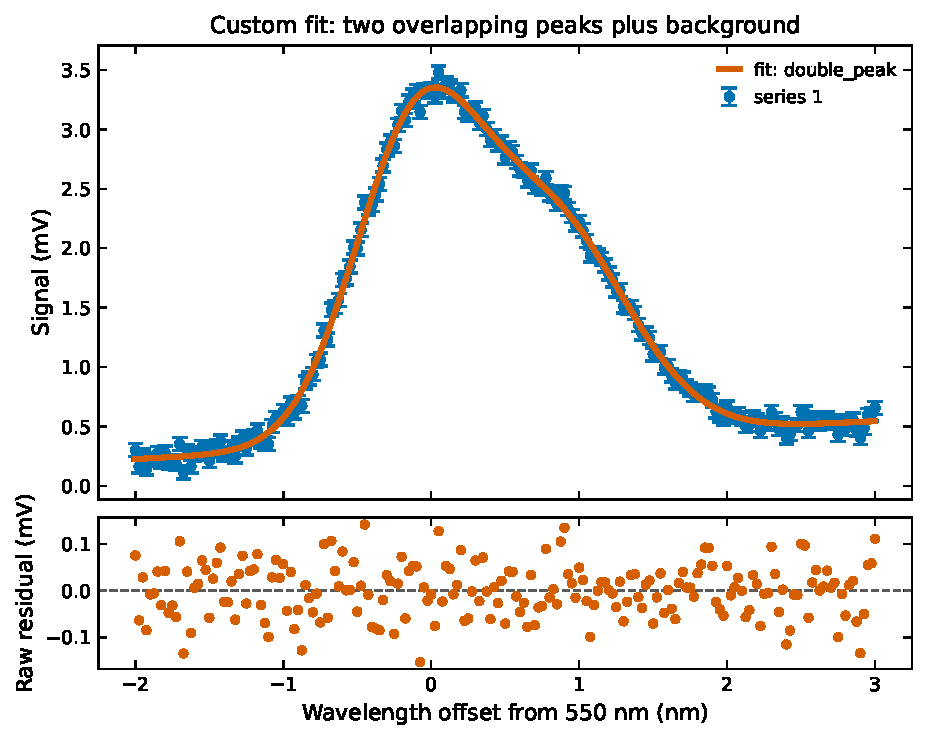
\includegraphics[width=0.9\linewidth,height=\textheight,keepaspectratio]{figures/05_double_peak.pdf}
\caption{Custom two-peak fit with background. The residual panel checks
the complete predicted signal against the observations.}
\end{figure}

\begin{figure}
\centering
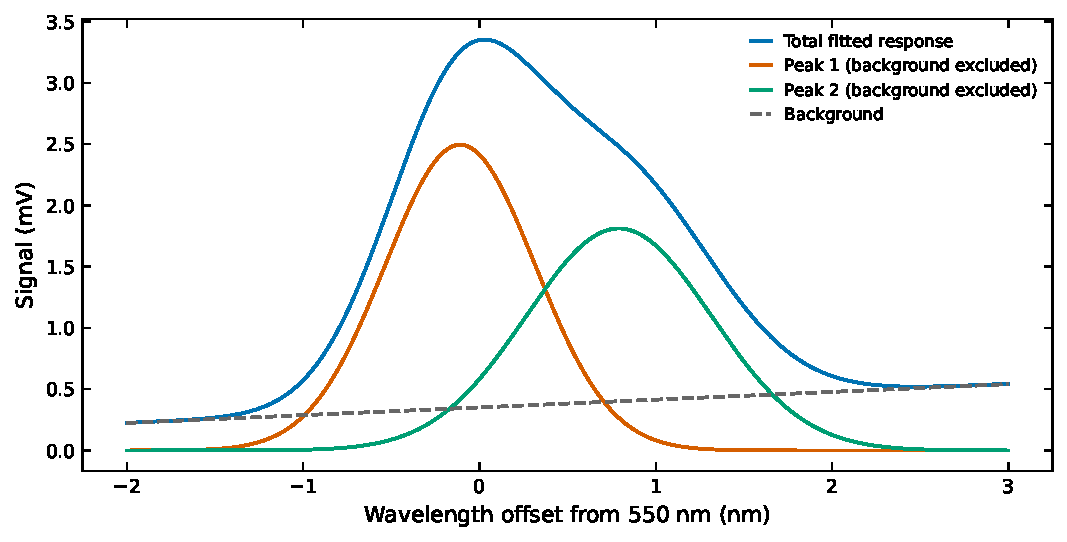
\includegraphics[width=0.9\linewidth,height=\textheight,keepaspectratio]{figures/05_components.pdf}
\caption{Decomposition of the fitted response. The orange and green
curves are individual baseline-subtracted Gaussian components; the
dashed line is the background, and the blue line is their total.}
\end{figure}

Component curves are model-derived contributions. They are not
separately measured spectra. Their apparent precision depends on the
model and the information available in the overlap region.

\Needspace{8\baselineskip}

\subsection{Inspect parameter
correlations}\label{inspect-parameter-correlations}

For fitted parameters \(\theta_i\) and \(\theta_j\), define

\begin{equation}\rho_{ij}=
\frac{(C_\theta)_{ij}}
{\sqrt{(C_\theta)_{ii}(C_\theta)_{jj}}}.\end{equation}

\begin{figure}
\centering
\pandocbounded{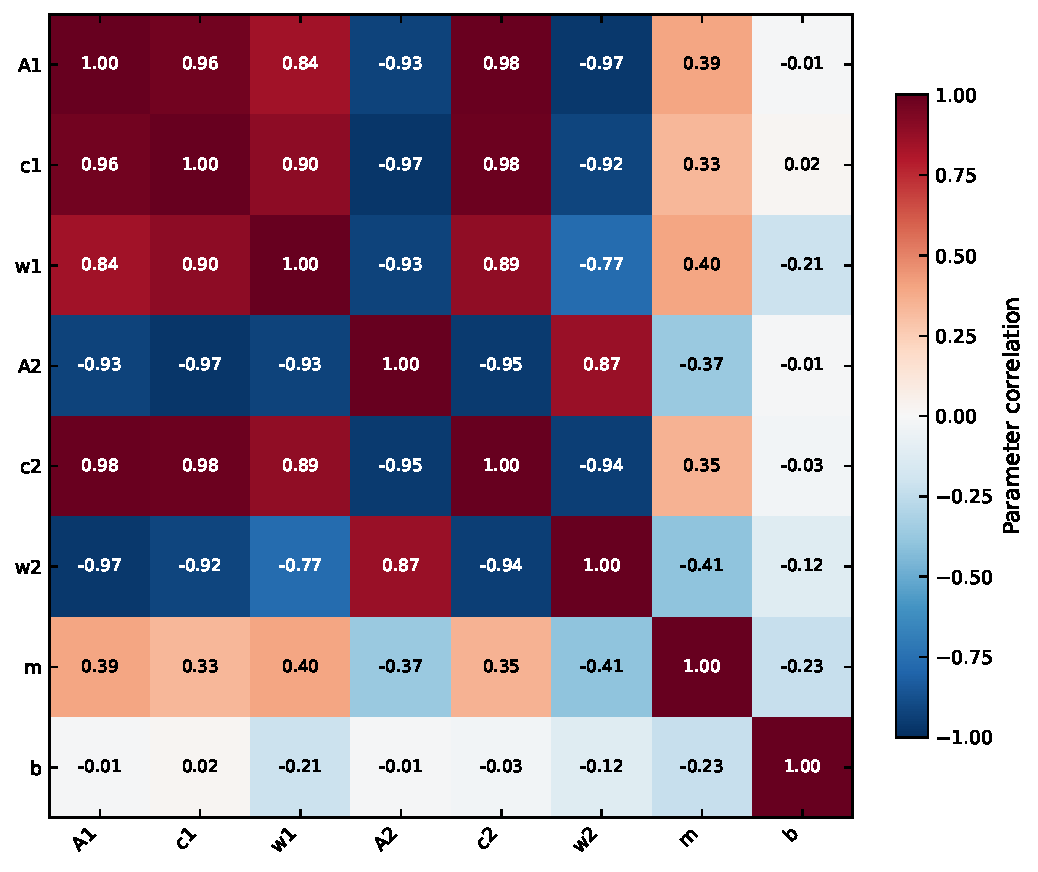
\includegraphics[keepaspectratio]{figures/05_correlations.pdf}}
\caption{Fitted parameter correlation matrix for the overlapping peaks.
Strong positive or negative entries show how parameters can compensate
for each other locally.}
\end{figure}

A large correlation is not automatically a failed fit. It explains why
uncertainty in a derived combination may differ substantially from the
sum of isolated parameter-error contributions.

Inspect \passthrough{\lstinline!result.jacobian\_rank!} and
\passthrough{\lstinline!result.jacobian\_condition!} alongside
\passthrough{\lstinline!identifiable!}. LabFit normalises Jacobian
columns for its condition diagnostic, reducing dependence on the units
of individual parameters. These are local checks; a nonlinear model may
also have distant alternatives.

\Needspace{8\baselineskip}

\subsection{Propagate the peak
separation}\label{propagate-the-peak-separation}

The peak separation is

\begin{equation}\Delta=c_2-c_1,\qquad
s_\Delta^2=s_{c_1}^2+s_{c_2}^2-2\,\mathrm{Cov}(c_1,c_2).\end{equation}

The shared reference wavelength cancels from the difference. For
absolute centres it would remain relevant, but an exact common
coordinate shift does not change separation.

\par\noindent\begin{minipage}{\linewidth}

\begin{lstlisting}[language=Python]
names = ("c1", "c2")
indices = [result.param_names.index(name) for name in names]
centre_covariance = result.covariance[np.ix_(indices, indices)]
separation, separation_error = propagate_errors(
    lambda c1, c2: c2 - c1,
    jacobian=lambda c1, c2: np.array([-1.0, 1.0]),
    covariance=centre_covariance,
    c1=result.params["c1"],
    c2=result.params["c2"],
)
\end{lstlisting}

\end{minipage}\par

\begin{longtable}[]{@{}llll@{}}
\toprule\noalign{}
Derived quantity & Estimate & Standard error & Unit \\
\midrule\noalign{}
\endhead
\bottomrule\noalign{}
\endlastfoot
Peak separation & 0.899532 & 0.0183 & nm \\
\end{longtable}

The extracted covariance follows the order \((c_1,c_2)\), matching both
function arguments and the gradient \((-1,1)\).

\textbf{Laboratory lesson:} overlapping components need more than a
successful optimiser status. Use defensible bounds, compare starting
values, inspect correlations and propagate the uncertainty of the
quantity you actually need.

\clearpage

\section{Complex example 6: correlated thermal
measurements}\label{complex-example-6-correlated-thermal-measurements}

\Needspace{8\baselineskip}

\subsection{Question and response
model}\label{question-and-response-model}

A sensor warms toward a new equilibrium after a temperature step. Nearby
readings share a fluctuating instrumental component. We ask:
\textbf{what time constant describes the response when measurement
errors are correlated?}

Use LabFit's \passthrough{\lstinline!exponential\_rise!} model:

\begin{equation}T(t)=T_0+A\left[1-\exp(-t/\tau)\right].\end{equation}

\begin{longtable}[]{@{}lll@{}}
\toprule\noalign{}
LabFit name & Meaning & Unit \\
\midrule\noalign{}
\endhead
\bottomrule\noalign{}
\endlastfoot
\passthrough{\lstinline!amplitude!} & Change from initial to final
temperature & degree C \\
\passthrough{\lstinline!tau!} & Response time constant & s \\
\passthrough{\lstinline!offset!} & Initial temperature & degree C \\
\end{longtable}

The asymptotic temperature is
\passthrough{\lstinline!offset + amplitude!}. At \(t=\tau\), the
temperature has completed \(1-\exp(-1)\), about 63 percent, of its total
rise.

There are 81 observations over 0 to 120 seconds. The generator uses
amplitude 12 degrees C, time constant 28 s and initial temperature 21
degrees C. Seed 606 controls the Gaussian noise draw.

The first rows of \href{data/thermal.csv}{the thermal CSV} are:

\begin{longtable}[]{@{}lll@{}}
\toprule\noalign{}
x & y & sigma \\
\midrule\noalign{}
\endhead
\bottomrule\noalign{}
\endlastfoot
0 & 21.0542 & 0.208806 \\
1.5 & 21.9012 & 0.208806 \\
3 & 22.4545 & 0.208806 \\
4.5 & 23.0992 & 0.208806 \\
6 & 23.6504 & 0.208806 \\
\end{longtable}

\Needspace{8\baselineskip}

\subsection{Supply measurement
covariance}\label{supply-measurement-covariance}

The measurement covariance uses an exponentially decaying correlation
plus independent instrument noise:

\begin{equation}(C_y)_{ij}=s_c^2\rho^{|i-j|}+s_n^2\delta_{ij},
\qquad s_c=0.20,\ s_n=0.06,\ \rho=0.78.\end{equation}

The standard deviations are in degrees C, so covariance entries are in
degrees C squared. The Kronecker delta \(\delta_{ij}\) is one on the
diagonal and zero elsewhere.

The CSV's \passthrough{\lstinline!sigma!} column gives marginal standard
deviations, \(\sqrt{(C_y)_{ii}}\), for inspection and for the
intentionally simplified comparison fit. The full matrix is supplied
separately in \href{data/thermal_covariance.csv}{the covariance CSV}.

\begin{figure}
\centering
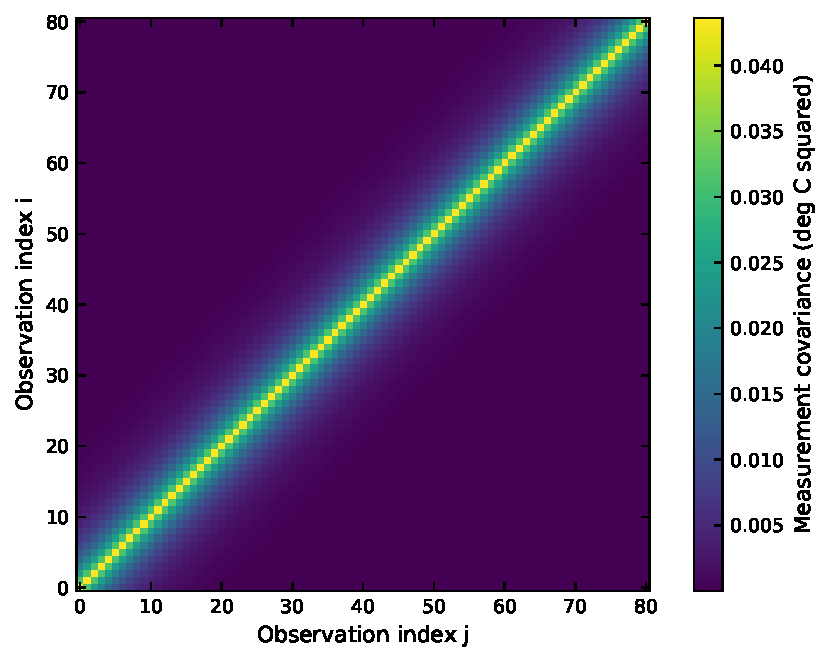
\includegraphics[width=0.9\linewidth,height=\textheight,keepaspectratio]{figures/06_covariance.pdf}
\caption{Measurement covariance for the thermal observations. Entries
decrease away from the diagonal because the shared noise correlation
decays with sample separation.}
\end{figure}

Covariance rows and columns correspond exactly to the observation order
in the measurement CSV. If you select or reorder observations, apply the
same selection or permutation to both covariance axes. Sorting the data
alone changes the stated error model.

LabFit requires a finite, symmetric, positive-definite measurement
covariance. An invalid or singular matrix is rejected before
optimisation. A covariance matrix has physical and statistical meaning;
adding an arbitrary diagonal term solely to avoid an error needs
justification.

\Needspace{8\baselineskip}

\subsection{Fit with and without
correlations}\label{fit-with-and-without-correlations}

\par\noindent\begin{minipage}{\linewidth}

\begin{lstlisting}[language=sh]
python examples/tutorial/example_06_correlated.py
\end{lstlisting}

\end{minipage}\par

\par\noindent\begin{minipage}{\linewidth}

\begin{lstlisting}[language=Python]
series = load_csv(data / "thermal.csv", label="Thermal step response")
covariance = np.loadtxt(data / "thermal_covariance.csv", delimiter=",")
initial = {"amplitude": float(series.y[-1] - series.y[0]), "tau": 30.0, "offset": float(series.y[0])}
bounds = {"amplitude": (0, 30), "tau": (1, 200), "offset": (10, 30)}
correlated = fit(
    series.x,
    series.y,
    sigma_cov=covariance,
    model="exponential_rise",
    p0=initial,
    bounds=bounds,
    absolute_sigma=True,
)
diagonal = fit(
    series,
    model="exponential_rise",
    p0=initial,
    bounds=bounds,
    absolute_sigma=True,
)
cholesky = np.linalg.cholesky(covariance)
whitened = solve_triangular(cholesky, correlated.residuals, lower=True)
chi2_from_residuals = float(whitened @ whitened)
\end{lstlisting}

\end{minipage}\par

The correlated fit passes only \passthrough{\lstinline!sigma\_cov!}; it
does not also pass scalar sigmas. The diagonal comparison uses the CSV's
marginal sigmas and assumes independent errors. Both fits use the same
response model, starting values, bounds and absolute covariance policy.

The initial amplitude comes from the observed change. The 30-second
starting time constant is a rough scale from the visible rise, and the
initial offset comes from the first observation.

\Needspace{6\baselineskip}

\subsubsection{Generalized least-squares
result}\label{generalized-least-squares-result}

\begin{longtable}[]{@{}llll@{}}
\toprule\noalign{}
Parameter & Estimate & Standard error & Unit \\
\midrule\noalign{}
\endhead
\bottomrule\noalign{}
\endlastfoot
\passthrough{\lstinline!amplitude!} & 11.7661 & 0.203 & degree C \\
\passthrough{\lstinline!tau!} & 27.3101 & 1.14 & s \\
\passthrough{\lstinline!offset!} & 21.1233 & 0.192 & degree C \\
\end{longtable}

Degrees of freedom: \textbf{78}; reduced chi-square: \textbf{0.8221};
chi-square p-value: \textbf{0.8709}. Converged: \textbf{True};
identifiable: \textbf{True}.

\Needspace{6\baselineskip}

\subsubsection{Diagonal-error
comparison}\label{diagonal-error-comparison}

\begin{longtable}[]{@{}llll@{}}
\toprule\noalign{}
Parameter & Estimate & Standard error & Unit \\
\midrule\noalign{}
\endhead
\bottomrule\noalign{}
\endlastfoot
\passthrough{\lstinline!amplitude!} & 11.7381 & 0.0934 & degree C \\
\passthrough{\lstinline!tau!} & 27.7915 & 0.535 & s \\
\passthrough{\lstinline!offset!} & 21.1972 & 0.0995 & degree C \\
\end{longtable}

Degrees of freedom: \textbf{78}; reduced chi-square: \textbf{0.8889};
chi-square p-value: \textbf{0.7478}. Converged: \textbf{True};
identifiable: \textbf{True}.

\begin{figure}
\centering
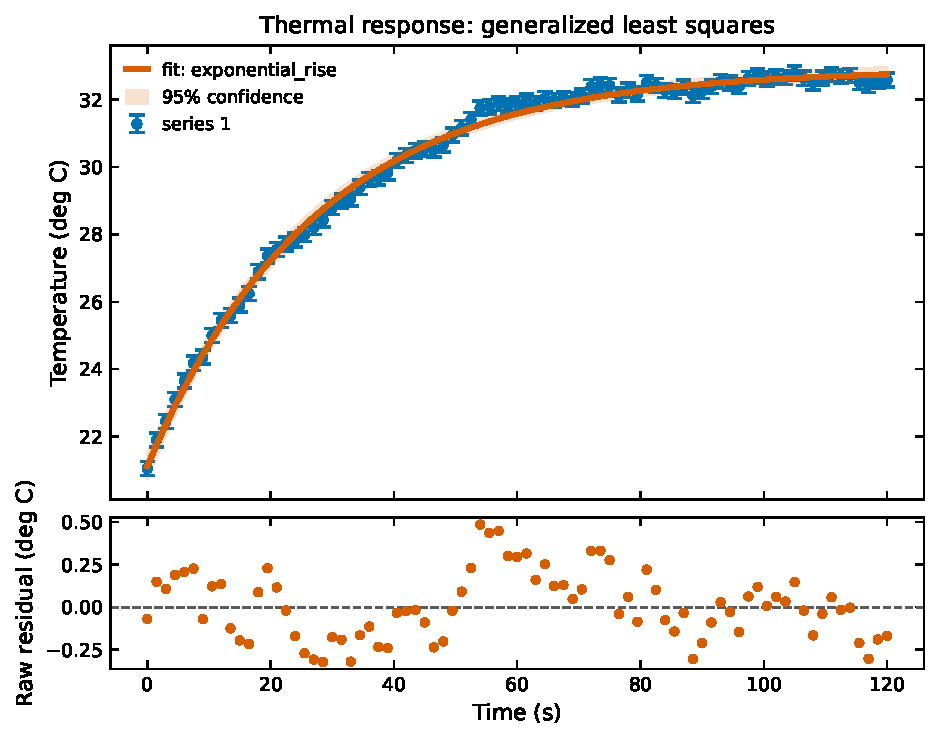
\includegraphics[width=0.9\linewidth,height=\textheight,keepaspectratio]{figures/06_correlated.pdf}
\caption{Thermal response fitted with full measurement covariance. Error
bars show marginal one-standard-deviation errors; they cannot themselves
display the correlations used in the fit.}
\end{figure}

The ratio of time-constant standard errors, correlated fit divided by
diagonal fit, is \textbf{2.13042}. For this dataset the correlated
analysis reports a larger uncertainty in the time constant. Repeated
adjacent readings provide less independent information than the diagonal
model assumes.

Correlation does not inflate every uncertainty by a universal factor.
Its effect depends on the covariance pattern and on which parameter
combination the data constrain. Estimates themselves can also change
because the weighting geometry changes.

\Needspace{8\baselineskip}

\subsection{Whiten the residuals}\label{whiten-the-residuals}

Generalized least squares minimises

\begin{equation}\chi^2=\boldsymbol{r}^T C_y^{-1}\boldsymbol{r}.\end{equation}

A Cholesky factor \(L\) satisfies \(C_y=LL^T\). Define whitened
residuals by solving \(L\boldsymbol{z}=\boldsymbol{r}\):

\begin{equation}\boldsymbol{z}=L^{-1}\boldsymbol{r},\qquad
\chi^2=\boldsymbol{z}^T\boldsymbol{z}.\end{equation}

Use a triangular solve rather than explicitly forming the matrix
inverse. The squared norm computed by the script is \textbf{64.1204}.
Multiplying LabFit's reported reduced chi-square by its degrees of
freedom gives \textbf{64.1204}. Their agreement checks that the
diagnostic uses the same covariance as the fit.

\begin{figure}
\centering
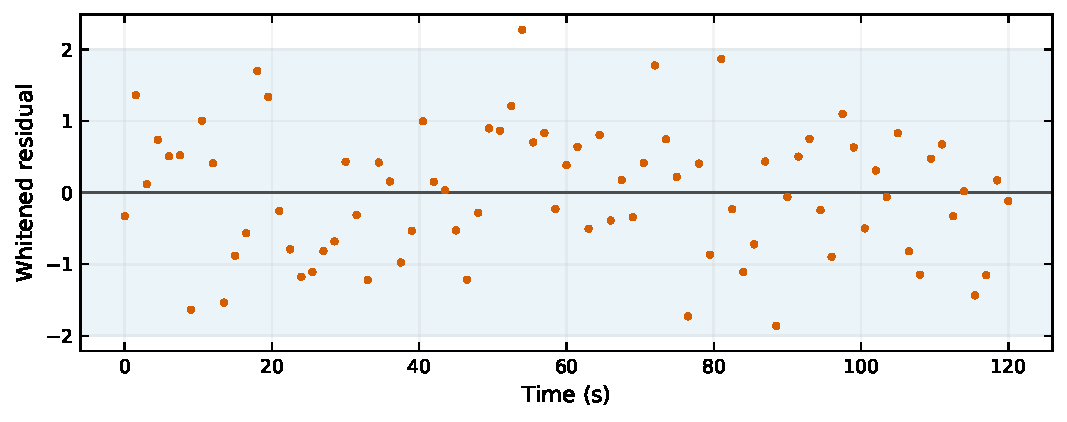
\includegraphics[width=0.9\linewidth,height=\textheight,keepaspectratio]{figures/06_whitened.pdf}
\caption{Whitened residuals for the thermal response. These
dimensionless values account for the supplied covariance; raw or
marginally standardized residuals would retain the noise correlations.}
\end{figure}

Whitening transforms the noise coordinates. The plotted time identifies
observation order, but each whitened coordinate can combine information
from several preceding observations. As with ordinary fitted residuals,
parameter estimation imposes constraints; do not treat every whitened
fitted residual as an independent, unconstrained Gaussian draw.

The chi-square p-value from the diagonal comparison assumes independent
errors. Since that assumption is false for this experiment, its
numerical value should not be interpreted as a calibrated
model-assessment probability.

\Needspace{8\baselineskip}

\subsection{Future observations need their own noise
model}\label{future-observations-need-their-own-noise-model}

A confidence band for the mean can use the fitted parameter covariance.
A prediction band additionally needs an error model for the future
observation. The training covariance describes the existing
observations, rather than an arbitrary new measurement.

LabFit therefore requires explicit
\passthrough{\lstinline!prediction\_sigma!} for a prediction band with
correlated training errors. Its prediction calculation assumes the
future error is independent of the fitted data. If the new reading
shares the same instrumental fluctuation, a marginal sigma alone does
not describe that dependence; a joint prediction calculation would be
needed.

\textbf{Laboratory lesson:} many closely spaced observations are not
necessarily many independent measurements. Preserve covariance through
fitting, diagnostics and interpretation.

\clearpage

\section{Reporting and
troubleshooting}\label{reporting-and-troubleshooting}

\Needspace{8\baselineskip}

\subsection{A defensible report}\label{a-defensible-report}

A useful analysis report contains the scientific question, equation and
parameter units; the observation source and preprocessing; the
uncertainty specification; starting values and bounds for nonlinear
fits; fitted estimates with errors; residual plots; and a discussion of
model limitations.

Report a derived quantity when it directly answers the scientific
question. For example, peak separation may be more relevant than eight
individual parameters. Keep full covariance and numerical precision in
machine-readable output, then round estimates and errors sensibly for
readers.

Avoid reporting long strings of digits as physical precision. A
conventional final laboratory summary rounds an uncertainty to one or
two significant figures and rounds its estimate to the corresponding
decimal place. The computed tables retain extra digits to support
reproduction.

These examples intentionally keep model selection modest. They do not
demonstrate robust regression, Poisson maximum likelihood, bootstrap
intervals, simultaneous bands or errors-in-variables fitting. Those
methods may be appropriate when the assumptions of this workflow fail.

\Needspace{8\baselineskip}

\subsection{Troubleshooting guide}\label{troubleshooting-guide}

\begin{longtable}[]{@{}
  >{\raggedright\arraybackslash}p{(\linewidth - 4\tabcolsep) * \real{0.3333}}
  >{\raggedright\arraybackslash}p{(\linewidth - 4\tabcolsep) * \real{0.3333}}
  >{\raggedright\arraybackslash}p{(\linewidth - 4\tabcolsep) * \real{0.3333}}@{}}
\toprule\noalign{}
\begin{minipage}[b]{\linewidth}\raggedright
Symptom
\end{minipage} & \begin{minipage}[b]{\linewidth}\raggedright
Check
\end{minipage} & \begin{minipage}[b]{\linewidth}\raggedright
Useful next step
\end{minipage} \\
\midrule\noalign{}
\endhead
\bottomrule\noalign{}
\endlastfoot
Fit does not converge & Starting values, units, bounds, model domain &
Plot the starting curve; choose a physically sensible scale \\
Converged fit leaves structured residuals & Missing baseline, curvature,
second component or drift & Revise the model based on experimental
knowledge \\
NaN parameter errors & Identifiability and degrees of freedom & Remove
redundant parameters or collect more informative data \\
Very large reduced chi-square & Model inadequacy, bad data or
underestimated errors & Inspect residuals and measurement procedure \\
Very small reduced chi-square & Error scale, overfitting, chance
fluctuation & Revisit errors; avoid automatic rescaling \\
Covariance rejected & Shape, ordering, finiteness, symmetry and positive
definiteness & Correct the covariance model or file alignment \\
Missing uncertainty warning & CSV columns and inference provenance &
Supply calibrated errors or choose explicit unweighted loading \\
Unexpected peak labels & Interchangeable components & Use defensible
centre windows or a clear labelling convention \\
\end{longtable}

A zero measurement sigma is invalid because it would claim infinite
precision. To exclude observations explicitly, use an appropriate data
mask or zero inverse-variance weights. Document exclusion decisions;
removing inconvenient residuals can bias both the fit and its apparent
goodness-of-fit.

Nonpositive degrees of freedom make residual-scale diagnostics
unavailable. More observations can help, but simply increasing the
number of nearly identical or heavily correlated measurements may add
little new information.

\Needspace{8\baselineskip}

\subsection{Compact API reference}\label{compact-api-reference}

\Needspace{6\baselineskip}

\subsubsection{Loading and fitting}\label{loading-and-fitting}

\par\noindent\begin{minipage}{\linewidth}

\begin{lstlisting}[language=Python]
from labfit import DataSeries, Fitter, fit, fit_multi
from labfit.io import load_csv

series = load_csv("measurements.csv", label="Experiment")
result = fit(series, model="linear", absolute_sigma=True)

# Equivalent array interface
result = fit(x, y, model="linear", sigma=errors, absolute_sigma=True)

# Covariance interface: supply covariance, without another error specification
result = fit(x, y, model="linear", sigma_cov=C_y, absolute_sigma=True)

# Reusable model configuration
fitter = Fitter(model="linear")
result = fitter(series, absolute_sigma=True)
\end{lstlisting}

\end{minipage}\par

Model names select built-in functions; a callable provides a custom
model. \passthrough{\lstinline!p0!} can map parameter names to starting
values. \passthrough{\lstinline!bounds!} can map names to lower/upper
tuples, using \passthrough{\lstinline!None!} for an unbounded side.
Initial values must lie inside the supplied bounds.

\Needspace{6\baselineskip}

\subsubsection{Reading results}\label{reading-results}

\begin{longtable}[]{@{}
  >{\raggedright\arraybackslash}p{(\linewidth - 2\tabcolsep) * \real{0.5000}}
  >{\raggedright\arraybackslash}p{(\linewidth - 2\tabcolsep) * \real{0.5000}}@{}}
\toprule\noalign{}
\begin{minipage}[b]{\linewidth}\raggedright
Attribute or method
\end{minipage} & \begin{minipage}[b]{\linewidth}\raggedright
Meaning
\end{minipage} \\
\midrule\noalign{}
\endhead
\bottomrule\noalign{}
\endlastfoot
\passthrough{\lstinline!params!} & Parameter-name to fitted-value
mapping \\
\passthrough{\lstinline!uncertainties!} & Parameter-name to
standard-error mapping \\
\passthrough{\lstinline!param\_names!} & Order of rows/columns in
parameter covariance \\
\passthrough{\lstinline!covariance!} & Local fitted-parameter
covariance \\
\passthrough{\lstinline!predict(x)!} & Model predictions at supplied x
values \\
\passthrough{\lstinline!residuals!} & Observations minus fitted
predictions \\
\passthrough{\lstinline!success!}, \passthrough{\lstinline!message!} &
Optimiser status and explanation \\
\passthrough{\lstinline!identifiable!} & Local reliability of separating
the parameters \\
\passthrough{\lstinline!jacobian\_rank!},
\passthrough{\lstinline!jacobian\_condition!} & Local Jacobian
diagnostics \\
\passthrough{\lstinline!dof!}, \passthrough{\lstinline!reduced\_chi2!},
\passthrough{\lstinline!p\_value!} & Degrees of freedom and weighted
diagnostics \\
\passthrough{\lstinline!residual\_variance!} & Raw residual scatter per
positive degree of freedom \\
\passthrough{\lstinline!series!} & Data and actual uncertainty
specification used in fitting \\
\end{longtable}

\Needspace{6\baselineskip}

\subsubsection{Plotting and propagation}\label{plotting-and-propagation}

\par\noindent\begin{minipage}{\linewidth}

\begin{lstlisting}[language=Python]
from labfit import plot_fit, plot_multi_fit
from labfit.utils import propagate_errors

plot = plot_fit(result, show_residuals=True, xlabel="Time (s)", ylabel="Signal (V)")
plot.save("fit.png")

plot = plot_fit(result, show_ci=True, ci_level=0.95)
plot = plot_fit(result, show_ci=True, prediction=True,
                ci_level=0.95, prediction_sigma=0.1)

value, error = propagate_errors(
    derived_function, jacobian=gradient_function,
    covariance=parameter_covariance, parameter_a=a, parameter_b=b,
)
\end{lstlisting}

\end{minipage}\par

\passthrough{\lstinline!prediction\_sigma!} can be a scalar or a
function of the plotted x grid. For varying future errors, use a
function rather than reusing a training array with a different shape.
Match the future-noise units to y.

For propagation, provide parameter values in the same order represented
by the covariance and returned gradient. The names in the final generic
example must match the arguments of your derived function.

\clearpage

\section{Reproduce, inspect and
adapt}\label{reproduce-inspect-and-adapt}

\Needspace{8\baselineskip}

\subsection{Recreate the observations}\label{recreate-the-observations}

The supplied CSV files are sufficient to run all examples. Regenerate
them only when you explicitly want to recreate the synthetic experiment:

\par\noindent\begin{minipage}{\linewidth}

\begin{lstlisting}[language=sh]
python examples/tutorial/generate_data.py
\end{lstlisting}

\end{minipage}\par

The generator stores its true parameters and noise model in
\href{data/manifest.json}{the manifest}. Each dataset has a fixed random
seed. The thermal covariance is written with extra precision to preserve
symmetry and numerical properties.

For a separate output directory:

\par\noindent\begin{minipage}{\linewidth}

\begin{lstlisting}[language=sh]
python examples/tutorial/generate_data.py --output path/to/data
python examples/tutorial/run_examples.py --data path/to/data --output path/to/results
\end{lstlisting}

\end{minipage}\par

The second command saves computed results and both figure formats in the
chosen output directory. It does not alter the observations.

\Needspace{8\baselineskip}

\subsection{Rebuild Markdown, LaTeX and
PDF}\label{rebuild-markdown-latex-and-pdf}

The document builder executes the examples using the supplied data,
inserts code and results into one authored Markdown template, and
converts that document to LaTeX. Pandoc handles conversion; Tectonic
compiles the PDF.

\par\noindent\begin{minipage}{\linewidth}

\begin{lstlisting}[language=sh]
python examples/tutorial/build_tutorial.py
\end{lstlisting}

\end{minipage}\par

Install Pandoc and Tectonic from their official distributions if they
are not available. A bundled Codex Tectonic is detected when present.
You can also choose the executable explicitly:

\par\noindent\begin{minipage}{\linewidth}

\begin{lstlisting}[language=sh]
python examples/tutorial/build_tutorial.py --tectonic /path/to/tectonic
python examples/tutorial/build_tutorial.py --markdown-only
\end{lstlisting}

\end{minipage}\par

The Markdown-only option needs the normal Python dependencies and
creates the same analysis figures and result tables. It does not require
the two document executables.

To edit the tutorial, change
\passthrough{\lstinline!tutorial.template.md!}, the example scripts or
\passthrough{\lstinline!style.tex!}, then rebuild. Generated Markdown
and LaTeX are deliverables rather than separate authoring sources. Keep
the \passthrough{\lstinline!figures/!} directory beside the LaTeX source
when compiling it.

\Needspace{8\baselineskip}

\subsection{What the checks establish}\label{what-the-checks-establish}

The integration checks regenerate the data in a temporary directory and
compare CSV contents. They verify that measurement covariance is
positive definite and aligned with marginal sigmas. They execute all six
analyses and check convergence, local identifiability and finite
uncertainties.

Recovery of synthetic truth is assessed with explicit tolerances: five
estimated standard errors plus a small absolute numerical floor. This is
a broad regression guard, rather than a requirement that every estimate
lie within one standard error. The seeds are fixed without selecting
them for especially favourable diagnostics.

The checks also verify the covariance contribution to peak-separation
uncertainty and the agreement between generalized least-squares
chi-square and the squared norm of whitened residuals. The deliberately
incomplete background-free model must retain its conspicuously worse
diagnostic.

The document checks ensure that referenced files exist and template
placeholders have been resolved. The PDF is compiled and rendered for
visual inspection of code, tables, plots and page transitions.

\par\noindent\begin{minipage}{\linewidth}

\begin{lstlisting}[language=sh]
python -m pytest tests/test_tutorial.py -q
\end{lstlisting}

\end{minipage}\par

These checks support reproducibility and catch common implementation
errors. They do not establish that the model assumptions are suitable
for an unseen real experiment.

\Needspace{8\baselineskip}

\subsection{Adapt the workflow to your
experiment}\label{adapt-the-workflow-to-your-experiment}

Start by replacing one CSV with your observations and explicit errors.
Confirm the column units, shape and ordering. Plot the observations
before choosing starting values. Write the simplest model supported by
the experimental mechanism, then inspect its residuals before
interpreting parameter errors.

If you add a derived quantity, write its formula, identify which fitted
parameters it depends on, and extract covariance in that same order. If
you add a covariance matrix, preserve observation alignment through
every selection step.

The tutorial's complete analyses are available as:

\begin{itemize}
\tightlist
\item
  \href{example_01_calibration.py}{Linear calibration}
\item
  \href{example_02_decay.py}{Exponential decay}
\item
  \href{example_03_single_peak.py}{Single peak with background}
\item
  \href{example_04_oscillators.py}{Repeated damped oscillations}
\item
  \href{example_05_double_peak.py}{Overlapping peaks}
\item
  \href{example_06_correlated.py}{Correlated thermal response}
\end{itemize}

For further API details, consult the repository's documentation:
\href{../../docs/quickstart.rst}{quickstart},
\href{../../docs/concepts.rst}{concepts} and
\href{../../docs/fitting-functions.rst}{fitting functions}. The material
in this tutorial is implemented against the current checkout, so the
executable examples remain the direct reference for these
demonstrations.

\end{document}
